%Balíčky
\documentclass[a4paper,11pt,twoside]{article}
\usepackage[utf8]{inputenc} %kodovani, abychom mohli jednoduse psat diakriticka pismena
\usepackage[czech]{babel}
\usepackage{pifont}
\usepackage{graphicx} %pro vkladani obrazku
\usepackage{color}
\usepackage{fancyhdr} %zahlavi a zapati
\usepackage{ifpdf}
\usepackage{booktabs}
\usepackage{subfigure}
\usepackage{titlesec}
\usepackage[multiple]{footmisc}
\usepackage[final]{pdfpages}    % pro vkládání PDF souborů
\usepackage{pdflscape}   % pro sazbu stránek naležato
\usepackage{color}       % pro zvýraznění textu barvou
\usepackage{multirow} 
\usepackage{amsmath}
\usepackage{sectsty}
\usepackage[justification=centering]{caption}
\usepackage[top=1.5cm, left=3cm, right=3cm, bottom=2cm, headheight=26pt, includeheadfoot]{geometry}
\usepackage[colorlinks=false,urlcolor=black]{hyperref}
\usepackage{xcolor}
\usepackage{listings}
\usepackage{array}
\usepackage{multirow}
\usepackage{hhline}
\usepackage{gensymb}
\usepackage{graphicx}
\usepackage{enumitem}
\usepackage{verbatim}
\usepackage{amssymb}
\hypersetup{
    colorlinks=true,
    linkcolor=black,
    filecolor=black,      
    urlcolor=black,
    citecolor=black
}
\allsectionsfont{\rmfamily} 

\sectionfont{\huge}
\subsectionfont{\LARGE}
\subsubsectionfont{\Large}

\def\author{Autoři: Bc. Linda Kladivová, Bc. Jana Špererová}
\def\nazevprace{DIGITÁLNÍ MODEL TERÉNU A JEHO ANALÝZY}

\begin{document}
\setcounter{page}{1}  % nastaví čítač stránek od stránky Úvod na stránku č. 7
\sloppy
\setlength{\parskip}{1pt}


%%  ÚVODNÍ STRÁNKA %%%%%%%%%%%%%%%%%%%%%%%%%%%%%%%%%%%%%%%%%%%%%%

\pagestyle{empty} % vypne číslování stránek na úvodní straně

\begin{center}
\renewcommand{\baselinestretch}{1.30} %zvetseni mezery mezi radky

\LARGE
\textsc{České vysoké učení technické v~Praze} \\
\textsc{Fakulta stavební} \\

\bigskip

\large
\textsc{PROGRAM GEODÉZIE A KARTOGRAFIE} \\
\textsc{OBOR GEOMATIKA} \\

\vspace{10ex}

\begin{figure}[hbt!] %vlozeni loga
\begin{center}

\includegraphics[width=7cm]{pictures/symbol_cvut_konturova_verze_cb.pdf} 
\end{center}
\end{figure}

\vspace{20ex}

\large
\textsc{\nazevprace} \\
\smallskip


\vspace{6ex}

\normalsize
\textsc{\author} \\
\bigskip
\normalsize
\textsc{Předmět: Algoritmy digitální kartografie a GIS} \\

\end{center}


%% 2. STRÁNKA OBSAHUJE ZADÁNÍ
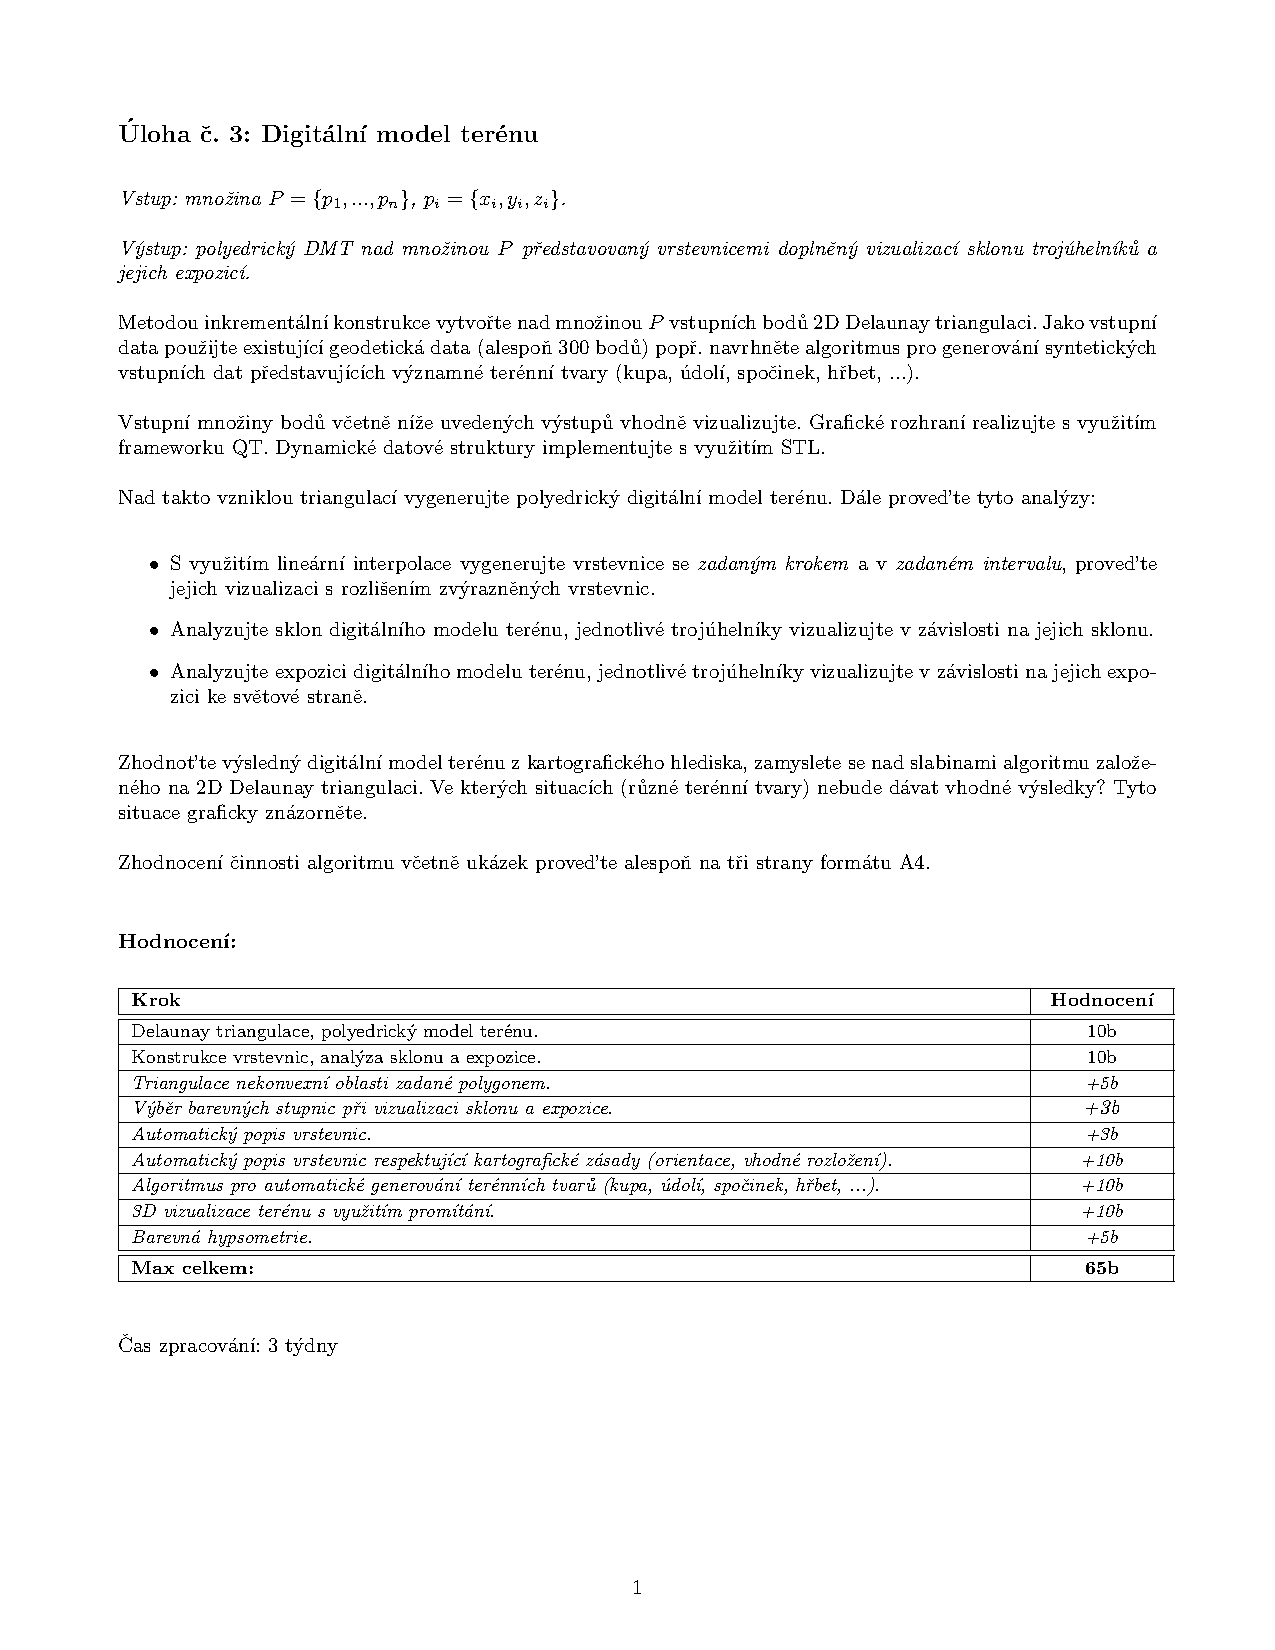
\includepdf{pictures/adkcv3}


%% 3. a 4. STRÁNKA = OBSAH A SEZNAM OBRAZKU %%%%%%%%%%%%%%%%%%%%%%%%%%%%%%%%%%
\renewcommand{\baselinestretch}{1.3} %zvetseni mezery mezi radky
\newpage
\tableofcontents %obsah

\newpage
\listoffigures %seznam obrázků
%\listoftables %seznam tabulek

\thispagestyle{empty}
\newcommand{\obrazek}[1]{(viz obr. \ref{#1})} %specialni reference na obrazek

\newpage
\fancyhead[RE, RO]{\fancyplain{}{\small \sl{POPIS A ROZBOR PROBLÉMU}}}
\pagestyle{fancy}

%% NASTAVENI VZHLEDU STRANEK (ZAHLAVI A ZAPATI)

\renewcommand{\baselinestretch}{1.4} %zvetseni mezery mezi radky

% zajistí, že se názvy kapitol a sekcí nebudou sázet velkými písmeny
\renewcommand{\sectionmark}[1]{\markright{\ #1}}

\fancyhf{} % smaže aktuální nastavení záhlaví a zápatí
\renewcommand{\headrulewidth}{0.4pt} % vrchní linka
\renewcommand{\footrulewidth}{0.4pt}  %  spodní linka
\addtolength{\voffset}{-0.4cm}

 %záhlaví
\fancyhead[LE, LO]{{
\includegraphics[width=1cm]{pictures/symbol_cvut_konturova_verze_cb.pdf} }
   {\textsc{\small {ČVUT v Praze}} }} %logo skoly
\fancyhead[RE, RO]{\nouppercase{\rightmark}}
   
 %zápatí
\fancyfoot[RO, LE]{{\textsc{\small \thepage}}}

\fancypagestyle{plain}{
  \fancyhead{} % na prázdných stránkách nechci záhlaví
  \renewcommand{\headrulewidth}{0pt} % ani linku
}


%% -------<<< 1. KAPITOLKA = Popis a rozbor problému >>>-------\\%%
\pagestyle{fancy}
\newpage
\vspace*{-1cm}
\section{Popis a rozbor problému}
\large
\renewcommand{\baselinestretch}{1.4}
\noindent
Cílem úlohy bylo vytvořit model terénu takový, který na podkladě trojúhelníkové Delaunayho sítě umožní tvorbu vrstevnic, sklonu terénu a expozici. \\
\indent Trojúhelníková síť je základem pro každý digitální model terénu. Nejčastěji se všechny analýzy snaží najít rovnostranné trojúhelníky tak, aby co nejlépe odpovídaly terénu, jenž mají znázorňovat. Jsou však metody, které dbají na uchování důležitých hran a jejich trojúhelníky mají nejrůznější úhly. \\
\indent Triangulace, v dnešní době však slouží při mnohem vícero věcích, než jen u kartografie. Například na základě triangulace se určuje na mobilech otisk prstu či známé „face ID“ a existuje mnoho dalších způsobů využití. Triangulací je hned několik, Delaunayho, kterou používáme pro řešení této úlohy je jednou z nejčastějších, ale pak je také Greedy triangulace, minimum Weight triangulace, datově závislé triangulace či Constrained triangulace. \\
\indent Analýza sklonu terénu je dnes využívána hojně na silnicích. Každý se jistě setkal se značkou, která znázorňuje sklon terénu a varuje řidiče, že je zde terén strmější, či prudší. Stejné sklony se používají i u znázornění terénu. \\
\indent Analýza expozice je dnes hojně využívá nejen při volbě míst, kam sázet, ale také třeba v umění. Když umělec nakreslí kvádr tak, že jdou vidět jen tři strany a vystínuje ho, ukazuje nám, jak na něj dopadá světlo. Jedna strana světlá, druhá tmavší a třetí nejtmavší. Stejně jako terén, na kopce nám krásně svítí, ale do nějakých úžin nám téměř nesvítí.

\subsection{Údaje o bonusových úlohách}
\large
\noindent
V rámci úlohy bylyi řešeny tři bonusové úlohy:
\begin{itemize}
\item Výběr barevných stupnic při vizualizaci sklonu a expozice
\item Automatický popis vrstevnic
\item Algoritmus pro automatické generování terénních tvarů
\end{itemize}


%% -------<<< 2. KAPITOLA = Popis použitých algoritmů >>>-------\\%%

\fancyhead[RE, RO]{\fancyplain{}{\small \sl{POPIS POUŽITÝCH ALGORITMŮ}}}
\newpage
\vspace*{-1cm}
\section{Popis použitých algoritmů}
\noindent
Obecně lze metody triangulace rozdělit podle více aspektů. Jedním aspektem je dělení triangulací dle geometrické konstrukce. Mezi tyto triangulace můžeme zařadit Greedy triangulace, Delaunay triangulace, Minimum Weight triangulace, Constrained triangulace (triangulace s povinnými hranami) a datově závislé triangulace. Dále můžeme triangulace dělit podle použitých kritérií, tedy na lokálně optimální triangulace, globálně optimální triangulace a multikriteriálně optimalizované triangulace. \\
\indent V této úloze byla naprogramována Delaunay triangulace pomocí metody inkrementální konstrukce. Další metody přímé konstrukce Delaunayho triangulace jsou např. metoda lokálního prohazování, inkrementálního vkládání, Divide and Conquer (rozděl a panuj) či Sweep Line (zametací přímka). Pro nepřímou konstrukci se využívají Voronoi diagramy, v praxi však tento způsob není používaný. Inkrementální kontrukce je vhodná pro vstupní množiny do 1 milionu bodů, pro větší množiny (do 50 milionů) se používá inkrementální vkládání. Pro ještě větší množiny je nutné použít metodu Divide and Conquer, která je však hodně náročná zhlediska implementace.
\large

\subsection{Delaunayho triangulace}
Je metoda pro vytvoření trojúhelníkové sítě, jakožto digitálního modelu terénu a lze ji využít v rovině i v prostoru.
Metoda funguje na principu hledání minimální opsané kružnice vedoucí bodem, nejvhodnějším k již vytvořené orientované hraně a to v její levé polorovině. Pokud takový bod existuje, změníme orientaci hrany a pokračujeme dále v hledání dalších bodů. \\
\indent Celý algoritmus má seznam hran – Active Edge List (AEL), ke kterým ještě nebyl nalezen třetí bod. Pokud nalezneme novou hranu, musíme se přesvědčit, zdali hrana s opačnou orientací již v seznamu není. Pokud ne, vložíme nově nalezenou hranu a hledáme další, pokud už je, hrana se nevloží. A pokud k nějaké hraně z AEL nalezneme třetí bod, hranu ze seznamu odstraníme. Celý algoritmus trvá, dokud seznam AEL není prázdný. \\

\newpage
Delaunayho triangulace musí splňovat následující vlastnosti:

\begin{enumerate}
\item Uvnitř opsané kružnice libovolného trojúhelníku triangulace neleží žádný jiný bod.
\item Maximalizuje minimální úhel v trojúhelníku.
\item Vůči kritériu minimálního úhlu je lokálně i globálně optimální.
\item Triangulace je jednoznačná, pokud čtyři body neleží na kružnici.
\end{enumerate}

\subsubsection{Slovní zápis algoritmu}
\begin{enumerate}
\item Nalezení pivota q s minimální souřadnicí X:  $ q = min(x_i) $ 
\item Hledání nejbližšího bodu k pivotovi: $ ||p_1 - q||_2 = min  $
\item Vytvoření první hrany: $ e = (q, p_1) $ 
\item Hledání Delaunay bodu: $ \underline{p} = argmin_{\forall p_i \in \sigma_L (e)} r'(k_i); k_i = (a, b, p_i); e = (a, b)$ 
\subitem Při nenalezení Delaunay bodu změna orientace: $ \nexists \underline{p} : e \leftarrow (p_1, q);$ go to 4. 
\item Vytvoření zbývajících hran trojúhelníka: $ e_2 = (p_1,  \underline{p}); e_3 = ( \underline{p} , q) $
\item Přidání hran trojúhelníka do DT:  $ DT \leftarrow e; DT \leftarrow e_2; DT \leftarrow e_3  $  
\item Přidání hran trojúhelníka do AEL (active edges list):  $ AEL \leftarrow e; AEL \leftarrow e_2; AEL \leftarrow e_3  $  
\item Dokud není AEL prázdný proveď:
\subitem Hledání Delaunay bodu k hraně z AEL (viz 4).
\subitem Pokud Delaunay bod existuje. $ if \exists  \underline{p}$
\subsubitem Vytvoření zbývajících hran trojúhelníku:   $ e_2 = (p_1,  \underline{p}); e_3 = ( \underline{p} , q) $
\subsubitem Pokud nová hrana není v AEL, přidej.
\end{enumerate}

\newpage
\subsection{Konstrukce vrstevnic}
Vrstevnici můžeme označit jako křivku, spojující body o stejné nadmořské výšce. Jinými slovy jde o křivku, která vznikne protnutím terénu vodorovnými rovinami. Vrstevnice dělíme na základní, které jsou ve vzdálenosti intervalu vrstevnic. Dále pak Hlavní nebo také Zvýrazněné, což bývá zpravidla každá 5. základní vrstevnice. Pak jsou vrstevnice doplňkové, které se nachází v různých částech intervalu, nejčastěji polovina či čtvrtina a nakonec vrstevnice pomocné, které slouží v místech, kde potřebujeme lépe naznačit terén a ostatní vrstevnice by tomu nestačily (lomy, sesuvy…). \\
\indent Vrstevnice, jejich vzhled i popis je dán skrze kartografické zásady. Základní vrstevnice kreslíme tenkou čarou, hlavní pak silnější čarou a doplňkové čárkovanou čarou. Jejich popis by měl být orientován tak, že vršek textu je směřován do kopce a naopak spodek textu je směřován z kopce. Popis bývá většinou barevný a silný, jako vrstevnice, kterou označuje a je potřeba aby vrstevnice byly popisovány rovnoměrně po celé zmapované oblasti. Nejčastěji se popisují pouze hlavní vrstevnice.\\
\indent Vrstevnice lze tvořit dvěmi způsoby. První z nich je za pomoci protínání trojúhelníkové sítě vodorovnými rovinami. Druhý pak za pomoci lineární interpolace, kdy je rozestup mezi dvěma body konstantní a tedy i jejich spád. Tato metoda byla použita při našem řešení.

\vspace{0.2cm}
\begin{figure}[hbt!] 
\begin{center}
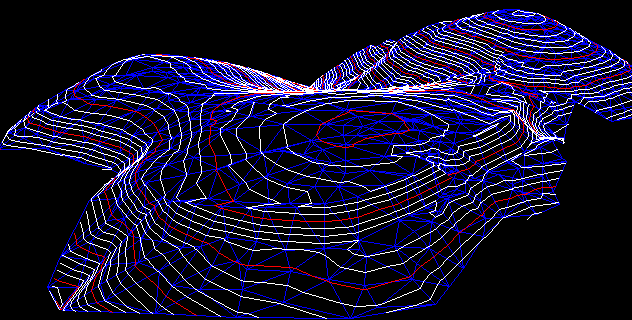
\includegraphics[width=15cm]{pictures/tin.png} 
\caption[Nepravidelná trojúhelníková síť (TIN) s vytvořenými vrstevnicemi]{Nepravidelná trojúhelníková síť (TIN) s vytvořenými vrstevnicemi \cite{tin}}
\label{fig:jar}
\end{center}
\end{figure}

\subsubsection{Slovní zápis algoritmu}
\begin{enumerate}
\item Pro všechny hrany trojúhelníku t: $ \forall e_i \in t: $ najdi průsečíky roviny a hrany. Může nastat několik případů:
\item Trojúhelník je celý v rovině vrstevnice - žádná vrstevnice se nekreslí.
\item Hrana náleží rovině vrstevnice z: $ (z - z_i) \cdot (z - z_{i+1}) = 0 \rightarrow e_i \in \rho $ (vrstevnice se vykreslí v příslušné hraně).
\item Hrana je průnikem roviny vrstevnice z: $ (z - z_i) \cdot (z - z_{i+1}) < 0 \rightarrow e_i \cap \rho $ (spočtou se průsečíky a ty se spojí vrstevnicovou hranou).
\subitem Výpočet polohových souřadnic: 
$$  x = \frac{(x_2 - x_1)}{(z_2 - z_1)} (z - z_1) + x_1 $$ 
$$  y = \frac{(y_2 - y_1)}{(z_2 - z_1)} (z - z_1) + y_1 $$ 
\subitem Vytvoř hranu tvořící vrstevnici.
\end{enumerate}

\subsection{Analýza sklonu DMT}
Sklon nám udává, zdali nám daný terén klesá, stoupá či zůstává neměnný. Máme-li dva normálové vektory (0,0,1) a normálový vektor roviny trojúhelníku z trojúhelníkové sítě, pak úhel mezi těmito normálovými vektory definuje sklon terénu.

\subsubsection{Slovní zápis algoritmu}
\begin{enumerate}
\item Pro všechny trojúhelníky triangulace: $ \forall t_i \in DT: $
\item Výpočet normálového vektoru roviny trojúhelníku:
$$  u_x = \Delta x_2, x_1; u_y = \Delta y_2, y_1; u_z = \Delta z_2, z_1;$$
$$  v_x = \Delta x_2, x_3; u_y = \Delta y_2, y_3; u_z = \Delta z_2, z_3;$$
 $$ n_t = (u_y \cdot v_z - u_z \cdot v_y)^2 - (u_x \cdot v_z - u_z \cdot v_x)^2  + (u_x \cdot v_y - u_y \cdot v_x)^2 $$
\item Výpočet sklonu: $ \varphi = arccos \frac{n_z}{|n_t|} $
\end{enumerate}

\vspace{0.2cm}
\begin{figure}[hbt!] 
\begin{center}
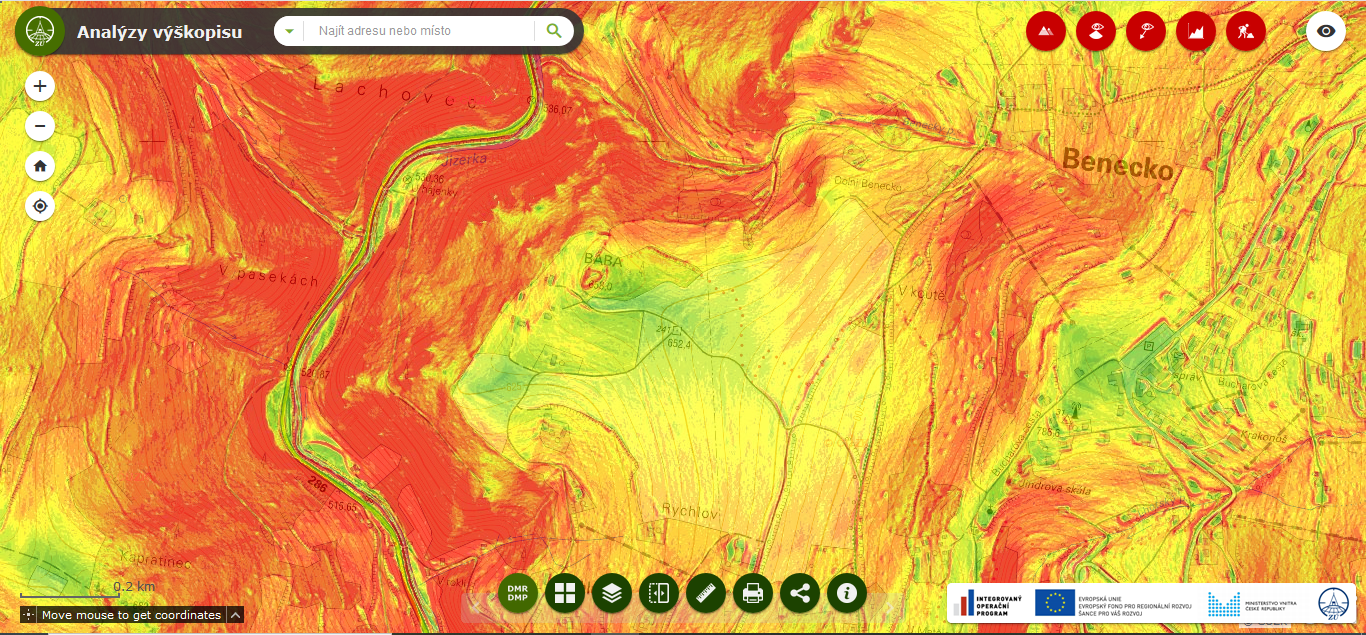
\includegraphics[width=15cm]{pictures/analyzy_sklon.png} 
\caption[Analýza sklonu svahu poskytovaná aplikací Analýzy výškopisu, jež spravuje Zeměměřický úřad]{Analýza sklonu svahu poskytovaná aplikací Analýzy výškopisu, jež spravuje Zeměměřický úřad \cite{analyzyCUZK}}
\label{fig:jar}
\end{center}
\end{figure}

\subsection{Analýza expozice DMT}
Expozice nám označuje orientaci terénu vzhledem ke světlu, tedy vzhledem k slunci. Jinými slovy nám říká, na jakou číst terénu dopadá kolik světla, kde je světla dostatek a kde je naopak stín. \\
\indent Pokud máme rovinu určenou souřadnicovými osami x a y a promítneme do ní normálový vektor roviny trojúhelníku, pak azimut tohoto průmětu definuje expozici terénu.


\subsubsection{Slovní zápis algoritmu}
\begin{enumerate}
\item Pro všechny trojúhelníky triangulace: $ \forall t_i \in DT: $
\item Výpočet x a y části normálového vektoru:
$$  u_x = \Delta x_2, x_1; u_y = \Delta y_2, y_1; u_z = \Delta z_2, z_1;$$
$$  v_x = \Delta x_2, x_3; u_y = \Delta y_2, y_3; u_z = \Delta z_2, z_3;$$
$$ n_x = (u_y \cdot v_z - u_z \cdot v_y) $$
$$ n_y = -(u_x \cdot v_z - u_z \cdot v_x) $$
\item Výpočet expozice: $ A =atan2( \frac{n_x}{n_y}) $
\end{enumerate}

\vspace{0.2cm}
\begin{figure}[hbt!] 
\begin{center}
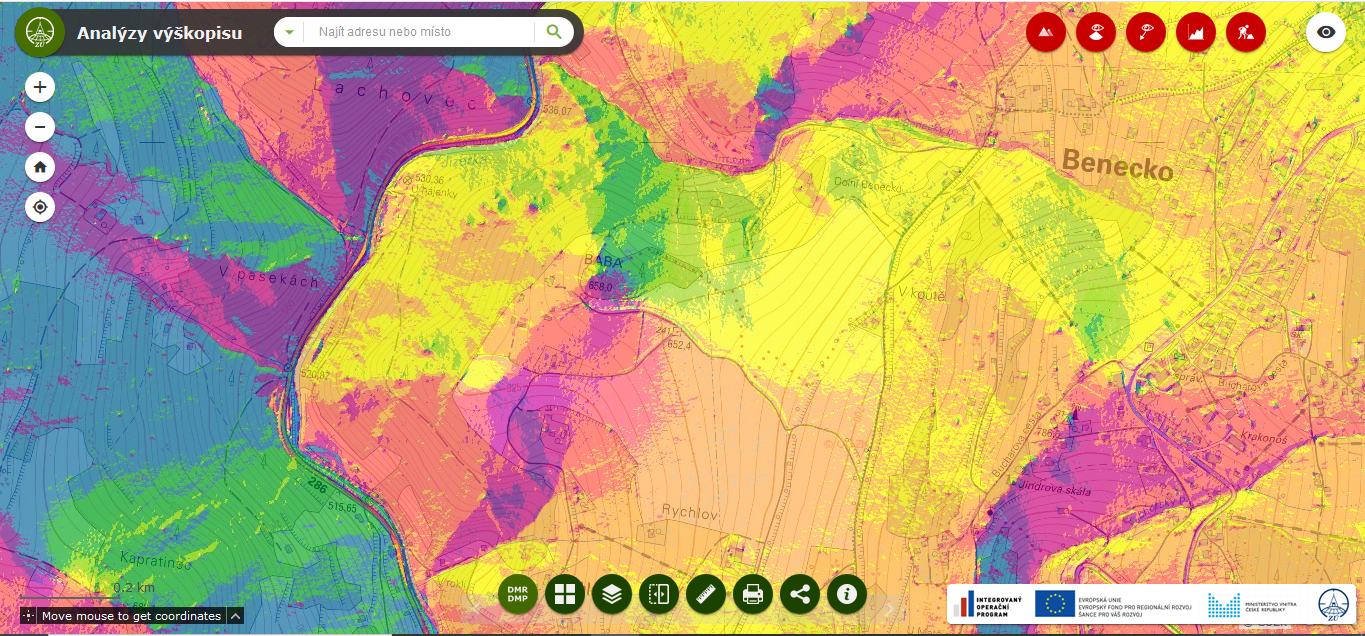
\includegraphics[width=15cm]{pictures/analyzy_orientace.PNG} 
\caption[Analýza expozice svahu poskytovaná aplikací Analýzy výškopisu, jež spravuje Zeměměřický úřad]{Analýza expozice svahu poskytovaná aplikací Analýzy výškopisu, jež spravuje Zeměměřický úřad \cite{analyzyCUZK}}
\label{fig:jar}
\end{center}
\end{figure}

%% -------<<< 2. KAPITOLKA = Informace o bonusových úlohách >>>-------\\%%
\fancyhead[RE, RO]{\fancyplain{}{\small \sl{INFORMACE O BONUSOVÝCH ÚLOHÁCH}}}
\section{Informace o bonusových úlohách}

\subsection{Výběr barevných stupnic}
V rámci této bonusové úlohy byly definovány barevné stupnice pro zobrazení sklonu a expozice. Byl vytvořen ComboBox, ve kterím je možné si vybrat buď panchromatickou škálu nebo barevnou škálu. Panchromatická škála pro sklon přiděluje černější barvu, pokud je sklon větší, naopak malé slkoly jsou teméř bíle. Nevýhodou trošku je, že data, která byla použita mají velmi malé sklony, tudíž barevný rozdíl v odstínech šedi není tak výrazný. Pro barevnou škálu pro sklon byly zvoleny odstíny barev od zelené (téměř rovina) po červenou (strmý svah). Inspirací pro volbu této barevné škály byla aplikace Analýzy výškopisu, jejímž provozovatelem je Zeměměřický úřad. \\
\indent Stupňové intervaly byly rovněž voleny podle schémata použitého ve výše zmíněné aplikaci při analýze \textit{Slope}, viz obrázek \ref{fig:analyzy_slope}. Aby byly dobře vidět i vrstevnice, bylo pracováno s průhledností. Složky RGB barev byly namíchány na webové stránce https://www.colorspire.com/rgb-color-wheel/. Samotné vytvoření barevných škál bylo implementováno ve třídě Draw, kde byly procházeny jednotlivé trojúhelníky Delaunayho triangulace a ke každému trojúhelníku podle spočtené analýzy a podle vybraného typu škály byla přiřazena konkrétní barva. Výběr barevných stupnic sklonu je nejlépe viditelný při analýzách nad generovanými terénními tvary. Na obrázcích \ref{fig:gentle_ridge_colorful_slope} a \ref{fig:gentle_ridge_panchromatic_slope}  je zobrazena analýzu sklonu nad spočinkem.

\vspace{0.2cm}
\begin{figure}[hbt!] 
\begin{center}
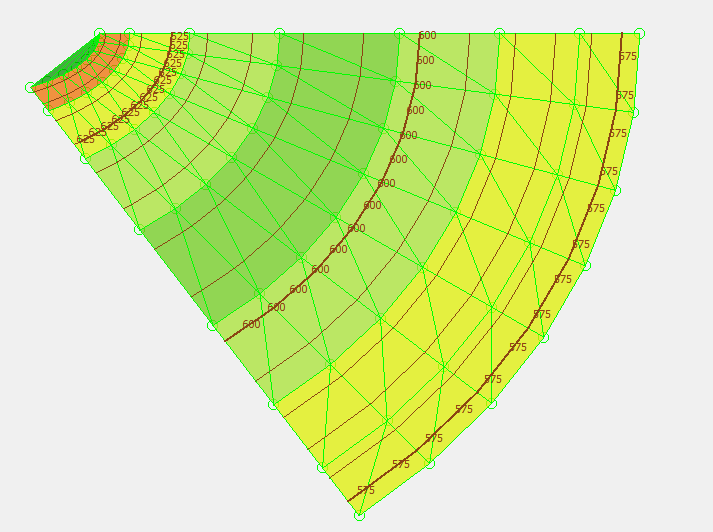
\includegraphics[width=12cm]{pictures/gentle_ridge_colorful_slope.PNG} 
\caption[Analýza sklonu nad spočinkem s využitím barevné škály]{Analýza sklonu nad spočinkem s využitím barevné škály}
\label{fig:gentle_ridge_colorful_slope}
\end{center}
\end{figure}

\begin{figure}[hbt!] 
\begin{center}
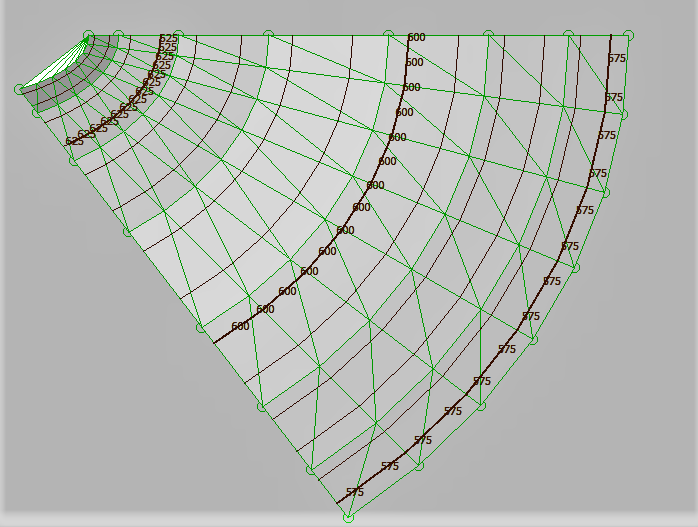
\includegraphics[width=12cm]{pictures/gentle_ridge_panchromatic_slope.PNG} 
\caption[Analýza sklonu nad spočinkem s využitím panchromatické škály]{Analýza sklonu nad spočinkem s využitím panchromatické škály}
\label{fig:gentle_ridge_panchromatic_slope}
\end{center}
\end{figure}


\begin{figure}[hbt!] 
\begin{center}
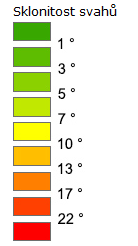
\includegraphics[width=3.3cm]{pictures/analyzy_slope.PNG} 
\caption[Stupňové intervaly v mapové aplikaci Analýzy výškopisu při analýze sklonu terénu ]{Stupňové intervaly v mapové aplikaci Analýzy výškopisu při analýze sklonu terénu}
\label{fig:analyzy_slope}
\end{center}
\end{figure}

\newpage
Pro vyznačení expozice byly v barevné škále voleny sytější barvy, která na sebe navazují. Inspirací pro stupňové intervaly byla barevná stupnice vytvořená pro analýzu \textit{Aspect} v programu ArcGIS, jež je znázorněna na následujícím obrázku \ref{fig:aspect}. 

\vspace{0.2cm}
\begin{figure}[hbt!] 
\begin{center}
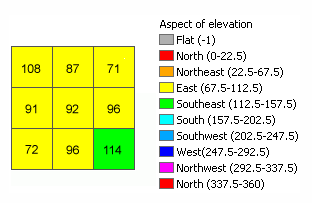
\includegraphics[width=11cm]{pictures/aspect.PNG} 
\caption[Intervaly expozice terénu v softwaru ArcGIS]{Intervaly expozice terénu v softwaru ArcGIS \cite{aspect}}
\label{fig:aspect}
\end{center}
\end{figure}

Barevní paleta byla volena podle schémata použitého v aplikaci Analýzy výškopisu, viz obrázek \ref{fig:analyzy_aspect}. Rovina nebyla uvažována.

\vspace{0.2cm}
\begin{figure}[hbt!] 
\begin{center}
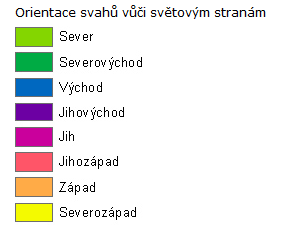
\includegraphics[width=7cm]{pictures/analyzy_aspect.PNG} 
\caption[Stupňové intervaly v mapové aplikaci Analýzy výškopisu při analýze orientace terénu ]{Stupňové intervaly v mapové aplikaci Analýzy výškopisu při analýze orientace terénu}
\label{fig:analyzy_aspect}
\end{center}
\end{figure}

\newpage
Obdobně byla vytvořena i panchromatická paleta, která nicméně v severním směru barevně nenavazuje, což není úplně štastné. Vhodnější je rozhodně pro analýzu orientace použít barevnou variantu.

Na obrázcích \ref{fig:gentle_ridge_colorful_aspect} a \ref{fig:gentle_ridge_panchromatic_aspect} můžeme vidět analýzu sklonu nad vygenerovaným spočinkem. Sklon se nejdříve snižuje a poté zase zvětšuje. Je patrné, že velká část spočinku se nachází v severovýchodním a východním směru.

\begin{figure}[hbt!] 
\begin{center}
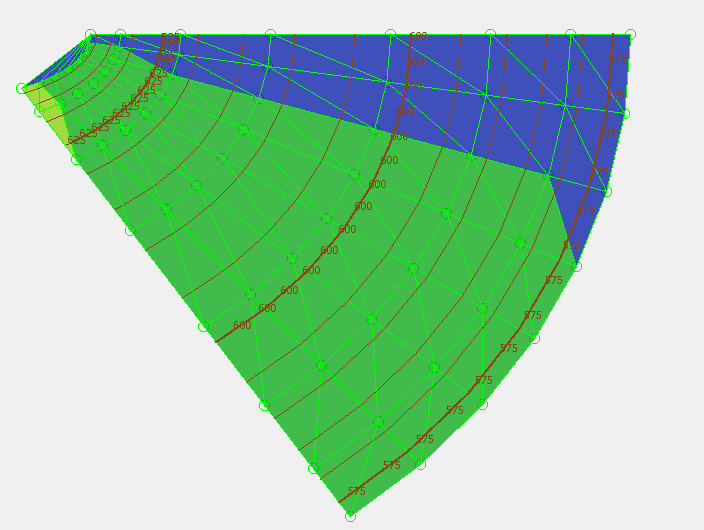
\includegraphics[width=12cm]{pictures/gentle_ridge_colorful_aspect.PNG} 
\caption[Analýza expozice nad spočinkem v barevné škále]{Analýza expozice nad spočinkem v barevné škále}
\label{fig:gentle_ridge_colorful_aspect}
\end{center}
\end{figure}

\vspace{0.2cm}
\begin{figure}[hbt!] 
\begin{center}
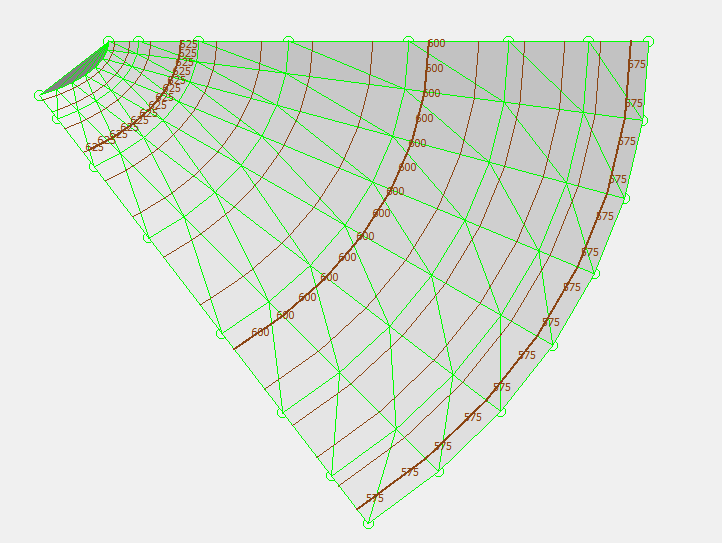
\includegraphics[width=15cm]{pictures/gentle_ridge_panchromatic_aspect.PNG} 
\caption[Analýza expozice nad spočinkem v panchromatické škále]{Analýza expozice nad spočinkem v panchromatické škále}
\label{fig:gentle_ridge_panchromatic_aspect}
\end{center}
\end{figure}

\subsection{Automatický popis vrstevnic}
Automatický popis vrstevnic byl vytvořen pro hlavní vrstevnice (každá pátá). Důležitým krokem bylo pozměnit funkci \textit{CreateContourLines}, aby nevracela pouze vektor hran vrstevnic, ale i vektor jednotlivých výšek. Tyto výšky pak byly pomocí funkce \textit{SetMainContours} převedeny do třídy \textit{Draw}, ve které byly využity přímo při vykreslování hlavních vrstevnic.\\ \indent Text byl umístěn do průměrných souřadnic mezi počátkem a koncem každé hrany hlavní vrstevnice. Pro umístění popisu byla použita funkce \textit{drawText}. Další vylepšení popisu vrstevnic, jako například natočení vzhledem k hraně, popis směřující hlavou do kopce, rovnoměrné rozložení kót po vrstevnici, či vynechání vrstevnice v místě popisu, řešeno nebylo. Popis hlavních vrstevnic je patrný z obrázku \ref{fig:gentle_ridge_panchromatic_aspect}.

\newpage
\vspace*{-1cm}
\subsection{Algoritmus pro automatické generování terénních tvarů}
V rámci bonusové úlohy byly vytvořeny algoritmy na automatické generování terénních tvarů. Konkrétně byly navrženy algoritmy na generování kupy, údolí, vodorovného hřbetu, sedla a spočinku. Navíc byla implementována možnost generování pravidelného gridu, jelikož takové rozmístění bodů má za následek nejednoznačnost DT, kdy žádné čtyři body nesmí ležet na kružnici. Všechny tyto algoritmy byly realizovány za využití velikosti mapového okna, a to tak, aby byly generovány pouze uvnitř této oblasti. Popis jednotlivých terénních útvarů byl použit ze středoškolských zápisek z předmětu Mapování.

\subsubsection{Kupa}
Jedná se o výrazně zaoblený vypuklý tvar. Povrch terénu klesá od vrcholu směrem na všechny strany. Tvarovou čárou je uzavřená křivka, která ohraničuje její vrchol a má kruhový, eliptický nebo nepravidelný tvar. V rámci naší aplikace je pro kupu zvoleno pojmenování \textbf{Hill}.

\vspace{0.2cm}
\begin{figure}[hbt!] 
\begin{center}
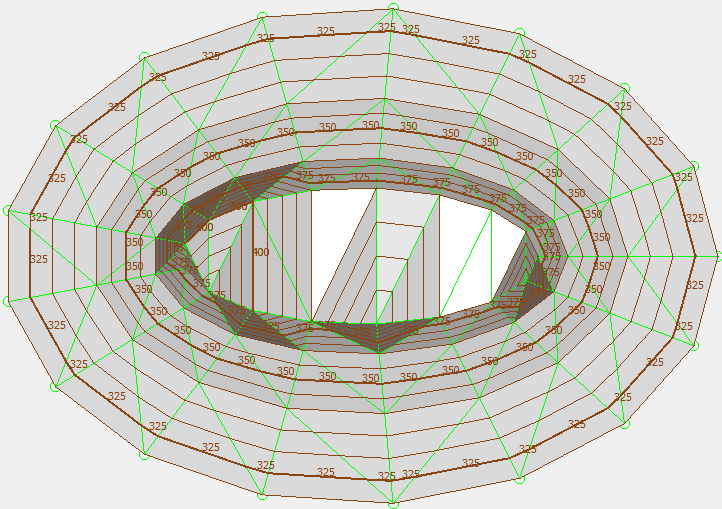
\includegraphics[width=12cm]{pictures/hill_panchromatic_slope.PNG} 
\caption[Vygenerovaná kupa s vrstevnicemi po analýze sklonu]{Vygenerovaná kupa s vrstevnicemi po analýze sklonu}
\label{fig:hill_panchromatic_slope}
\end{center}
\end{figure}

\indent Kupa byla generována pomocí několika elips, jejichž střed je vrcholem kupy. Elipsa s větším poloměrem má menší výšku Z, pro klesání byl zvolen krok 20. Vygenerovaná kupa je zobrazena na obrázku \ref{fig:hill_panchromatic_slope}.
$$
X = X_0 + a * cos(\phi)
$$
$$
Y = Y_0 + b * sin(\phi)
$$
$$
Z = Z_0 - j* 20
$$



\subsubsection{Údolí}
Jedná se o terénní útvar tvořící protáhlou vhloubenou plochu, která je tvořena působením vody nebo ledovci. V rámci aplikace je použito označení \textbf{Valley}.

\vspace{0.2cm}
\begin{figure}[hbt!] 
\begin{center}
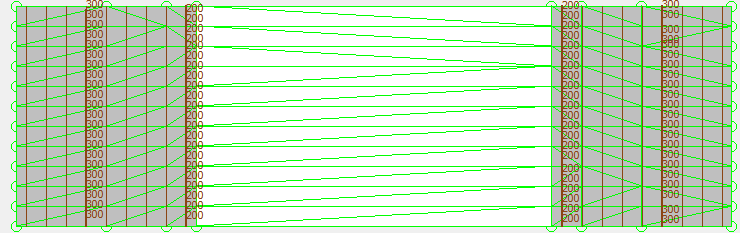
\includegraphics[width=11cm]{pictures/valley_panchromatic_slope.PNG} 
\caption[Vygenerované údolí s vrstevnicemi po analýze sklonu]{Vygenerované údolí s vrstevnicemi po analýze sklonu}
\label{fig:valley_panchromatic_slope}
\end{center}
\end{figure}

\indent Pro údolí byly vygenerovány přímky od nichž se v zadaném kroku vytváří nové přímky s konstantně stoupající hodnotou výšky. V uvedených vzorcích jsou p1 a p2 označení pro vzniklé přímky.Vygenerované údolí je zobrazeno na obrázku \ref{fig:valley_panchromatic_slope}.
$$
X_{p1} = X_0 + a
$$
$$
Y_{p1} = Y_0 + i * 10
$$
$$
Z_{p1} = Z_0 + a
$$
$$
X_{p2} = X_0 - a
$$
$$
Y_{p2} = Y_0 + i * 10
$$
$$
Z_{p2} = Z_0 + a
$$

\subsubsection{Vodorovný hřbet}
Jedná se o protáhlý vypuklý terénní tvar, jehož vrcholová část je zaoblená. V aplikace je pojmenován jako \textbf{Ridge}. Hřbet byl generován podobným způsobem jako údolí, s tím rozdílem, že výška postupně nestoupá, ale klesá.  Vygenerovaný vodorovná hřbet je zobrazen na obrázku \ref{fig:ridge_panchromatic_slope}.
$$
X_{p1} = X_0 + a
$$
$$
Y_{p1} = Y_0 + i * 10
$$
$$
Z_{p1} = Z_0 - a
$$
$$
X_{p2} = X_0 - a
$$
$$
Y_{p2} = Y_0 + i * 10
$$
$$
Z_{p2} = Z_0 - a
$$

\vspace{0.2cm}
\begin{figure}[hbt!] 
\begin{center}
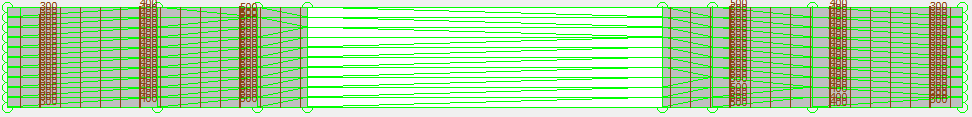
\includegraphics[width=12cm]{pictures/ridge_panchromatic_slope.PNG} 
\caption[Vygenerovaný vodorovný hřbet s vrstevnicemi po analýze sklonu]{Vygenerovaný vodorovný hřbet s vrstevnicemi po analýze sklonu}
\label{fig:ridge_panchromatic_slope}
\end{center}
\end{figure}

\subsubsection{Sedlo}
Tento terénní útvar označuje nejnižší plochu mezi dvěma terénními tvary, např. kupami. Stýkají se v něm dvě hřbetnice a dvě údolnice. Vbíhají do něj dvě plochy vypuklé s ubývajícím spádem kolmo na hřbetnici a vybíhají z něj dvě plochy vhloubené s přibývajícím spádem. V aplikace je použito označení \textbf{Saddle}. \\
\indent Generování sedla zahrnovalo vygenerování dvou kup a dvou prohlubní. Podstatné bylo rozmístění. Vlevo a vpravo od středu mapového okna byly generovány prohlubně, nahoře a dole kupy. Středy těchto terénních tvarů byly zvoleny napevno vzhledem ke středu mapového okna. Následně byly kolem těchto středů generovány elipsy s klesající/rostoucí výškou. Vygenerované sedlo je zobrazeno na obrázku \ref{fig:saddle_panchromatic_slope}. Můžeme si všimnout, že zvláště u vrcholů a prohlubní jsou výsledné vrstevnice generovány chybně. Mohla by pomoci možnost vložení povinných hran.\\

Tvorba elips u kupy:
$$
X = X_0 + i * rand\%(70) * cos(j*\phi) + rand\%(20)
$$
$$
Y =  Y_0 + i * rand\%(70) * sin(j*\phi) + rand\%(20)
$$
$$
Z = Z_0 - i * 50
$$

Tvorba elips u prohlubně:
$$
X = X_0 + i * rand\%(70) * cos(j*\phi) + rand\%(20)
$$
$$
Y =  Y_0 + i * rand\%(70) * sin(j*\phi) + rand\%(20)
$$
$$
Z = Z_0 + i * 50
$$

\vspace{0.2cm}
\begin{figure}[hbt!] 
\begin{center}
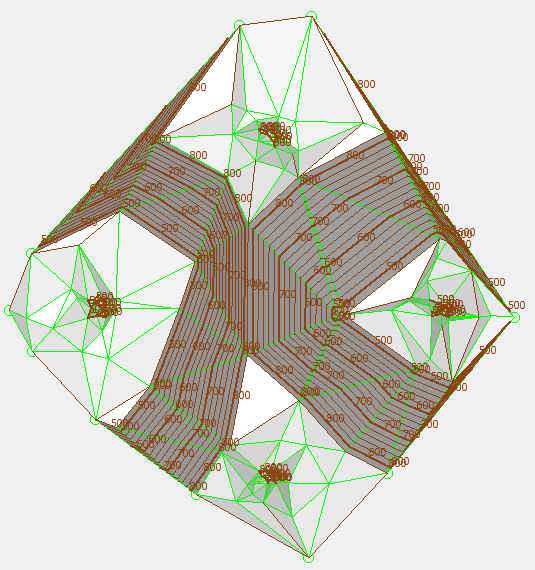
\includegraphics[width=12cm]{pictures/saddle_panchromatic_slope.PNG} 
\caption[Vygenerovanéí sedlo s vrstevnicem po analýze sklonui]{Vygenerované sedlo s vrstevnicemi po analýze sklonu}
\label{fig:saddle_panchromatic_slope}
\end{center}
\end{figure}

\newpage
\vspace*{-1cm}
\subsubsection{Spočinek}
Tento název označuje část hřbetu vyvýšeniny, kde hřbetnice přechází do mírnějšího sklonu, tj. plocha spočinku je oproti zbytku svahu méně skloněná nebo i vodorovná. tvarová čára se skládá ze dvou křivek -- jedna ohraničuje vbíhající vypuklou plochu, druhá ohraničuje vybíhající plochu. Rozestupy ve směru spádu se nejprve plynuje zvětšují a pak zase změnšují. V aplikaci lze spočinek vygenerovat pod názvem \textbf{Gentle Ridge}. \\
\indent Algoritmus na tvorbu spočinku je nejsložitější. Rozmezí úhlů, v kterých se generují elipsy je omezeno, tak aby výsledný útvar vytvářel šedesáti-stupňový vějíř. Je náhodně vygenerován vrchol, od kterého se pak vytváří části elips. Polovina elips je tvořena se zvyšujícím se poloměrem, tedy rozestupy vrstevnic se plynuje zvětšují. Další polovina vrstevnic je tvořena se snižujícím se poloměrem, tedy rozestupy ve směru spádu se plynule zmenšují. Počet elips je pevně daný, generování vrcholu a počtu bodů v elipsách je náhodné. Výškové rozdíly mezi jednotlivých elipsami jsou stejné, co se mění je pouze rozestup mezi nimi. Vygenerovaný spočinek je zobrazen na obrázku \ref{fig:gentle_ridge_panchromatic_slope}.

\vspace{0.2cm}
\begin{figure}[hbt!] 
\begin{center}
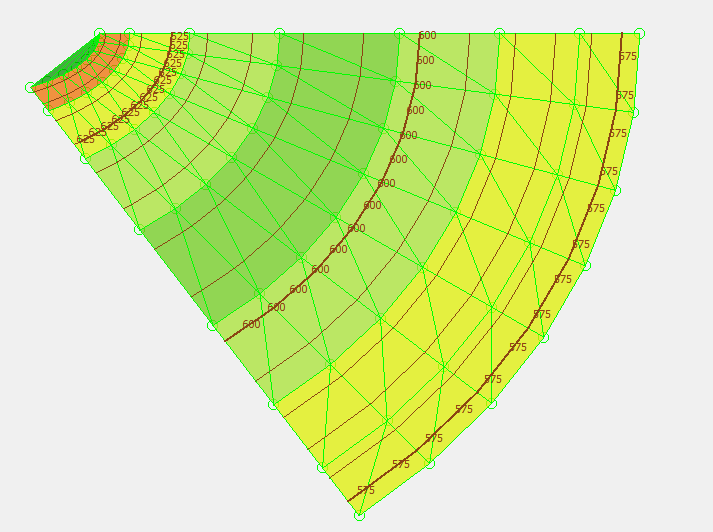
\includegraphics[width=12cm]{pictures/gentle_ridge_colorful_slope.PNG} 
\caption[Vygenerovaný spočinek s vrstevnicemi po analýze sklonu]{Vygenerovaný spočinek s vrstevnicemi po analýze sklonu}
\label{fig:gentle_ridge_colorful_slope}
\end{center}
\end{figure}

\newpage
\vspace*{-1cm}
\subsubsection*{Grid}
Aby bylo možné dobře demostrovat nejednoznačnost DT, byla naprogramována tvorba čtvercové mřížky. Nejeznačnost je však dobře patrná i u analýz nad hřbetem nebo údolím v nejvyšší resp. nejnižší části. Na obrázcích \ref{fig:grid_slope}, \ref{fig:grid_aspect}  je vidět nejednoznačnost hledání nejmenší opsané kružnice. Proto se může stát, že výsledné výpočty nebudou správné. V tomto případě však výsledné analýzy vycházejí správně.

\vspace{0.2cm}
\begin{figure}[hbt!] 
\begin{center}
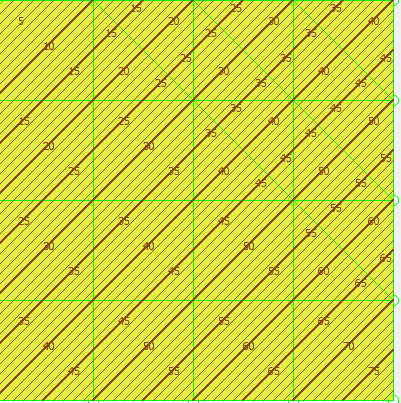
\includegraphics[width=7cm]{pictures/grid_colorful_slope.PNG} 
\caption[Vygenerovaná mřížka po analýze sklonu]{Vygenerovaná mřížka po analýze sklonu}
\label{fig:grid_slope}
\end{center}
\end{figure}

\vspace{0.2cm}
\begin{figure}[hbt!] 
\begin{center}
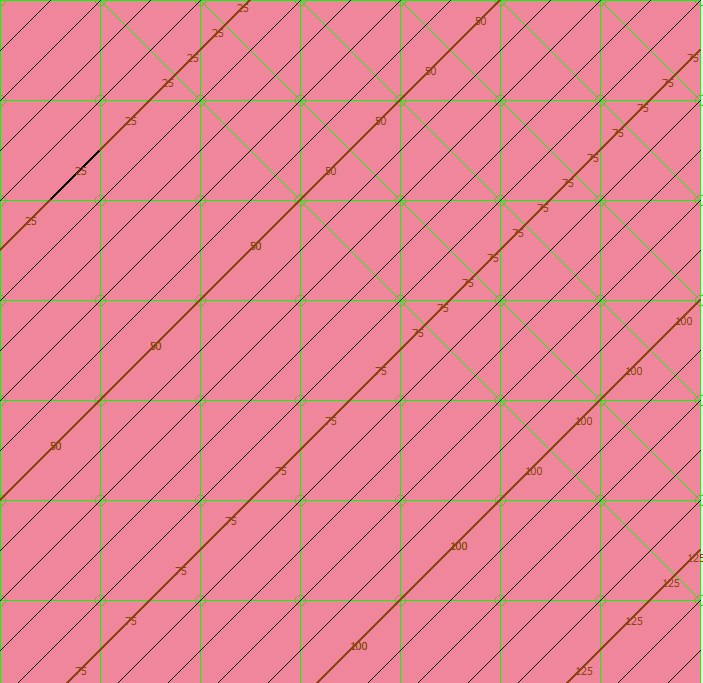
\includegraphics[width=7cm]{pictures/grid_colorful_aspect.PNG} 
\caption[Vygenerovaná mřížka po analýze expozice]{Vygenerovaná mřížka po analýze expozice}
\label{fig:grid_aspect}
\end{center}
\end{figure}

%% -------<<< 3. KAPITOLA = Vstupní  data >>>-------\\%%
\newpage
\fancyhead[RE, RO]{\fancyplain{}{\small \sl{VSTUPNÍ A VÝSTUPNÍ DATA}}}

\vspace*{-1cm}
\section{Vstupní data}
Vstupní data tvoří analyzovaná skupina bodů datového typu $std::vector<QPoint3D>$, která je vygenerována po stisku tlačítka \textit{Generate Points}. Tento generátor vytváří pomocí funkce \textit{rand} množiny významných terénních útvarů s předem definovaným počtem vrcholů. Druhým možným vstupem je zadání bodů kursorem myši (viz obrázek \ref{fig:contours_with_description}). Třetím možným vstupem je import skupiny bodů datového typu $std::vector<QPoint3D>$ ze souboru.  \\
Vzor vstupních dat YXZ ve formátu .txt je:
\begin{center}
845562.622	    998320.147     827.354\\
845560.329	    998321.145     826.989\\
845561.871	    998330.141     825.856\\ 
845562.564	    998329.139     827.546\\
\end{center}

\vspace{0.2cm}
\begin{figure}[hbt!] 
\begin{center}
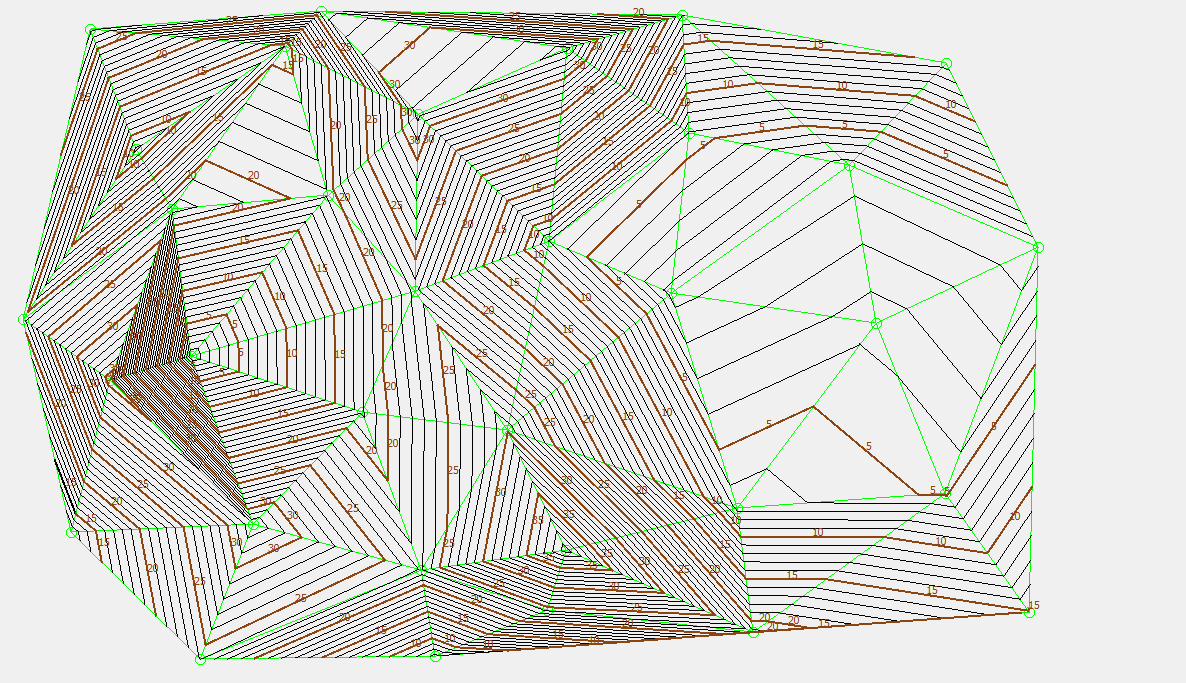
\includegraphics[width=11cm]{pictures/contours_with_description.png} 
\caption[Ukázka Delaunay modelu nad body zadanými kursorem myši]{Ukázka Delaunay modelu nad body zadanými kursorem myši}
\label{fig:contours_with_description}
\end{center}
\end{figure}

%% -------<<< 4. KAPITOLA = Výstupní data >>>-------\\%%
\section{Výstupní data}
Výstupem je grafická aplikace, která na vstupních datech vytvoří Delaunayho triangulaci. Nad touto triangulací je pak možné vykreslit vrstevnice s automatickým popisem hlavních vrstevnic a analyzovat sklon či expozici terénu.

%% -------<<< 5. KAPITOLA = Ukázka aplikace >>>-------\\%%
\newpage
\fancyhead[RE, RO]{\fancyplain{}{\small \sl{UKÁZKA APLIKACE}}}

\vspace*{-1cm}
\section{Ukázka aplikace}
\noindent
\large
Do této kapitolky je zahrnuto několik ukázek aplikace a výstupů, které lze přímo v aplikaci uložit jako obrázek. V pravé části aplikace může být měněn rozestup vrstevnic. V pravé horní části aplikace je možné importovat soubor s připravenými souřadnicemi. Analýzy takového souboru jsou zobrazeny na obrázcích \ref{fig:data_slope} a \ref{fig:data_aspect}.

\vspace{0.2cm}
\begin{figure}[hbt!] 
\begin{center}
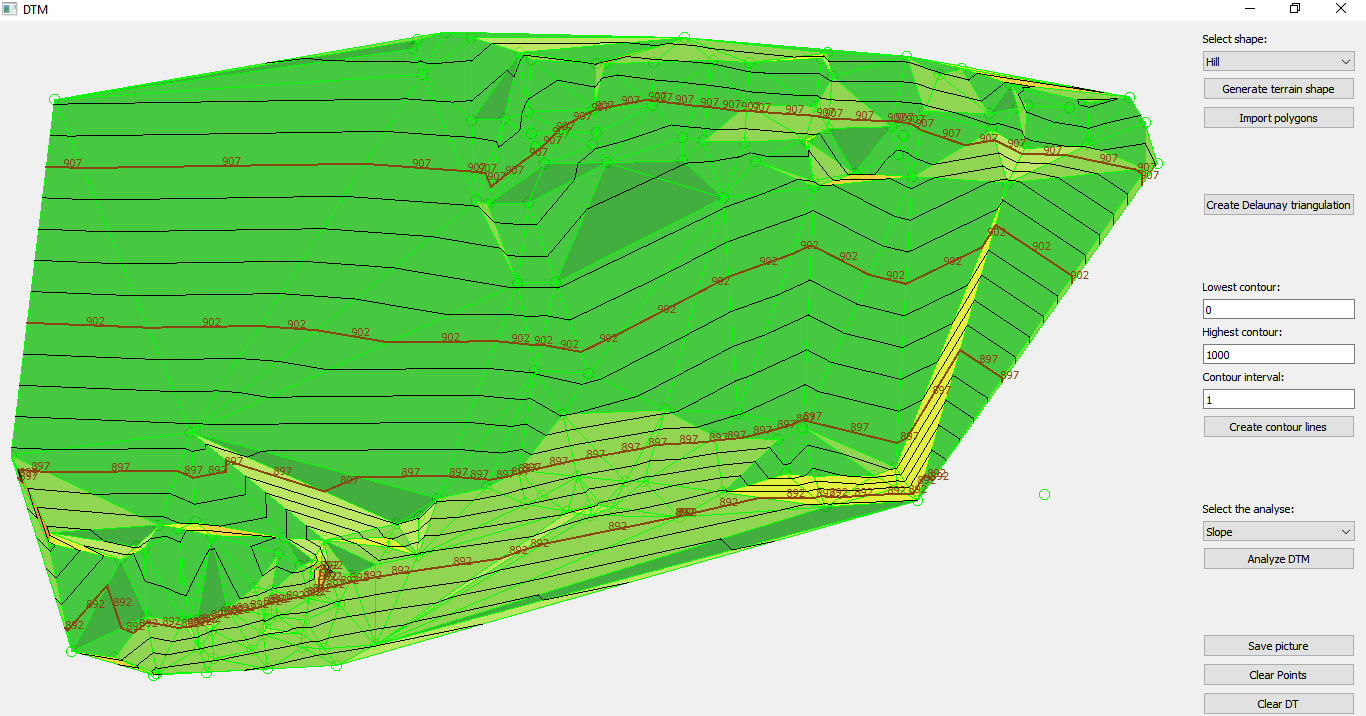
\includegraphics[width=13cm]{pictures/data_slope.PNG} 
\caption[Analýza sklonu nad testovacími geodetickými daty ze souboru]{Analýza sklonu nad testovacími geodetickými daty ze souboru}
\label{fig:data_slope}
\end{center}
\end{figure}

\begin{figure}[hbt!] 
\begin{center}
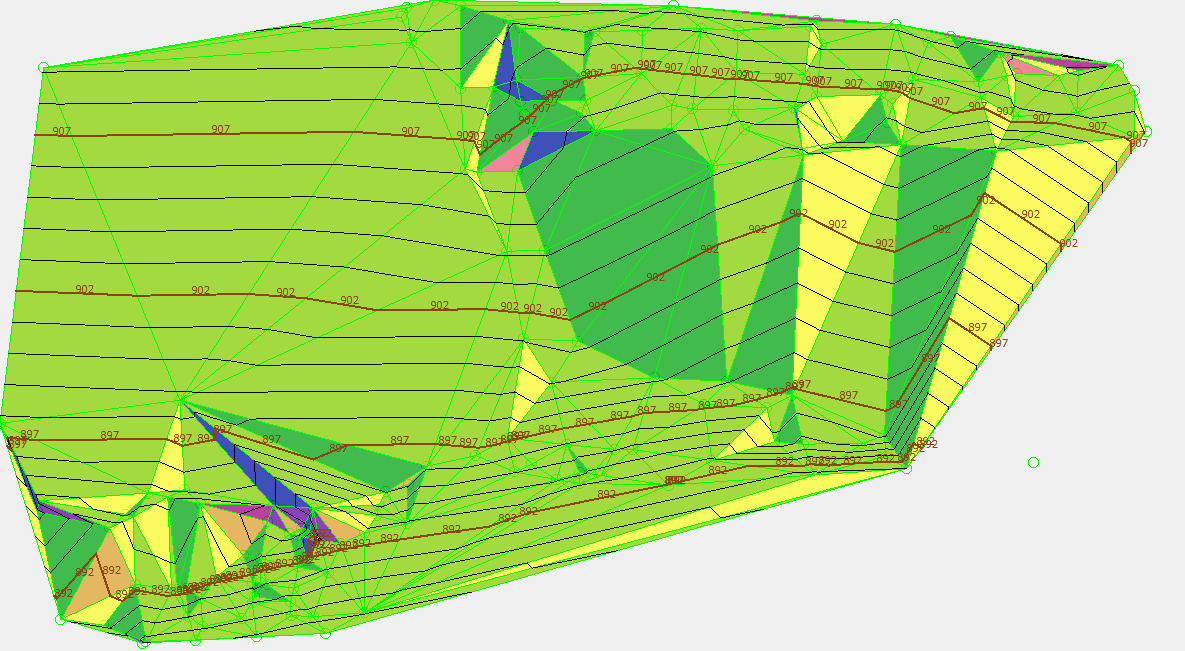
\includegraphics[width=13cm]{pictures/data_aspect.PNG} 
\caption[Analýza expozice nad testovacími geodetickými daty ze souboru]{Analýza expozice nad testovacími geodetickými daty ze souboru}
\label{fig:data_aspect}
\end{center}
\end{figure}

\begin{figure}[hbt!] 
\begin{center}
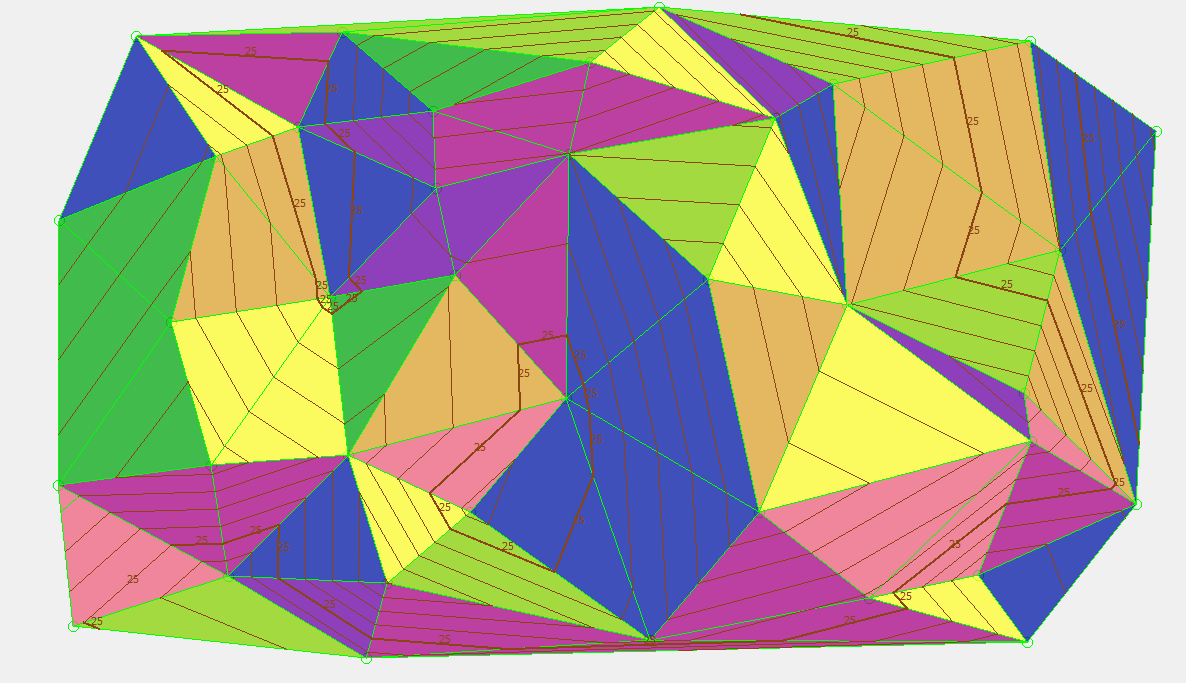
\includegraphics[width=15cm]{pictures/dtm_colorful_aspect.PNG} 
\caption[Analýza expozice v barevné škále nad body označenými kursorem myši]{Analýza expozice v barevné škále nad body označenými kursorem myši}
\label{fig:dtm_colorful_aspect}
\end{center}
\end{figure}

\begin{figure}[hbt!] 
\begin{center}
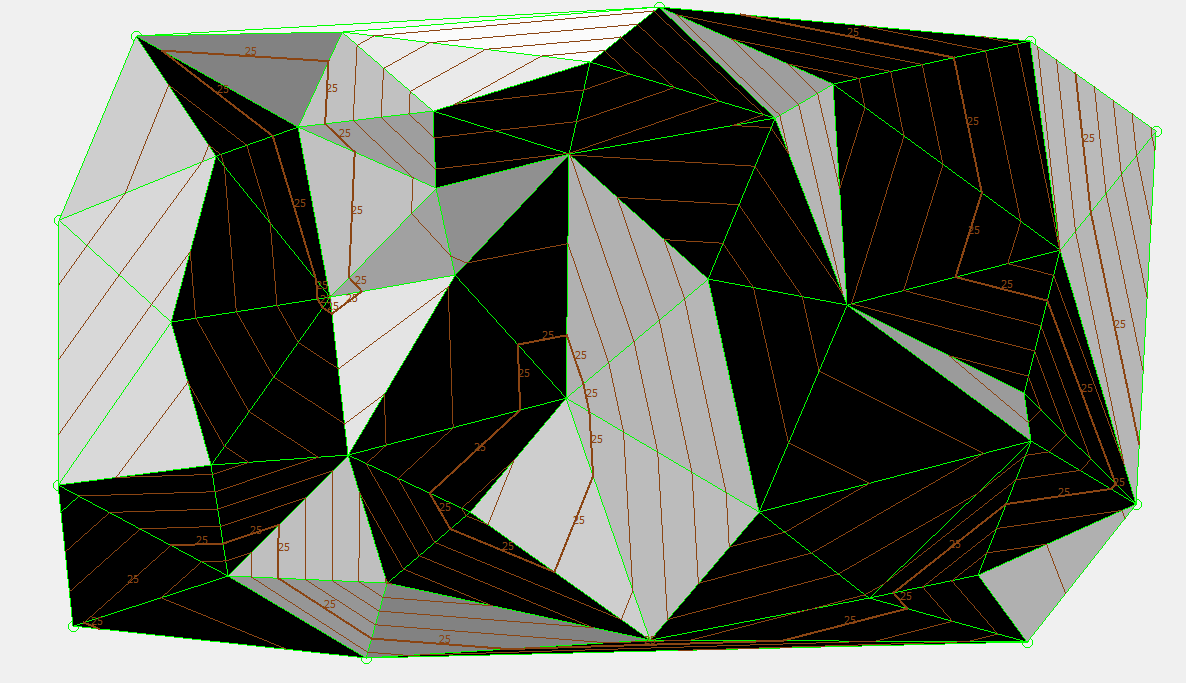
\includegraphics[width=15cm]{pictures/dtm_panchromatic_aspect.PNG} 
\caption[Analýza expozice v panchromatické škále nad body označenými kursorem myši]{Analýza expozice v panchromatické škále nad body označenými kursorem myši}
\label{fig:dtm_panchromatic_aspect}
\end{center}
\end{figure}

\begin{figure}[hbt!] 
\begin{center}
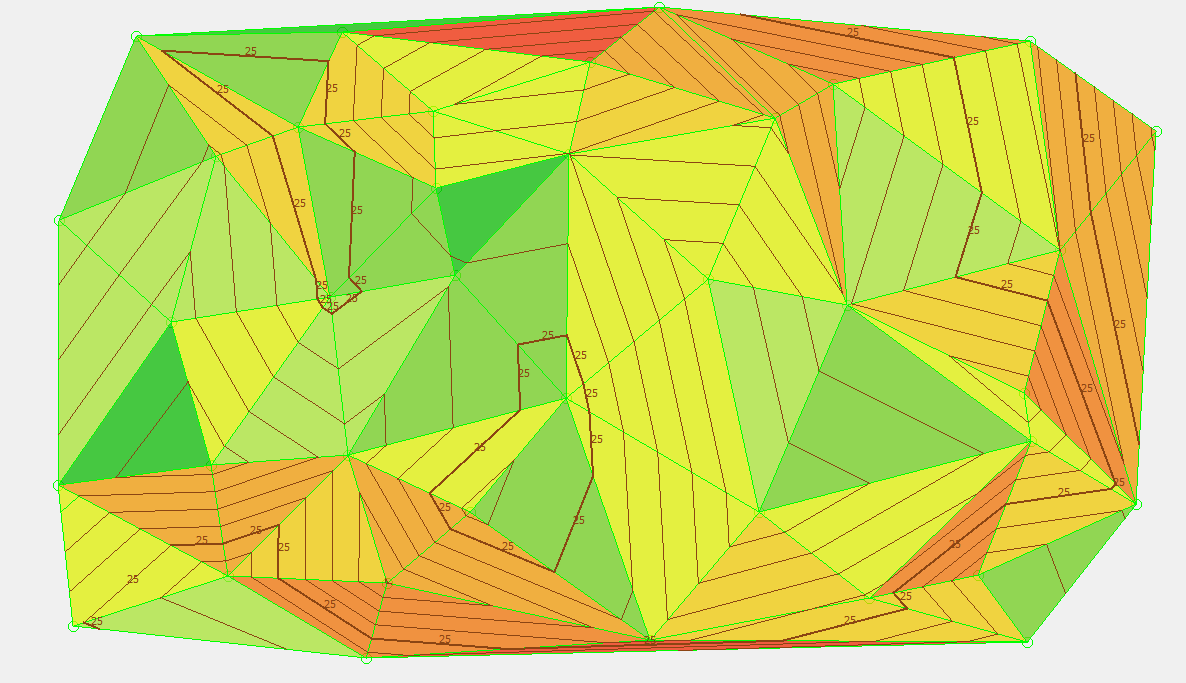
\includegraphics[width=15cm]{pictures/dtm_colorful_slope.PNG} 
\caption[Analýza sklonu v barevné škále nad body označenými kursorem myši]{Analýza sklonu v barevné škále nad body označenými kursorem myši}
\label{fig:dtm_colorful_slope}
\end{center}
\end{figure}

\begin{figure}[hbt!] 
\begin{center}
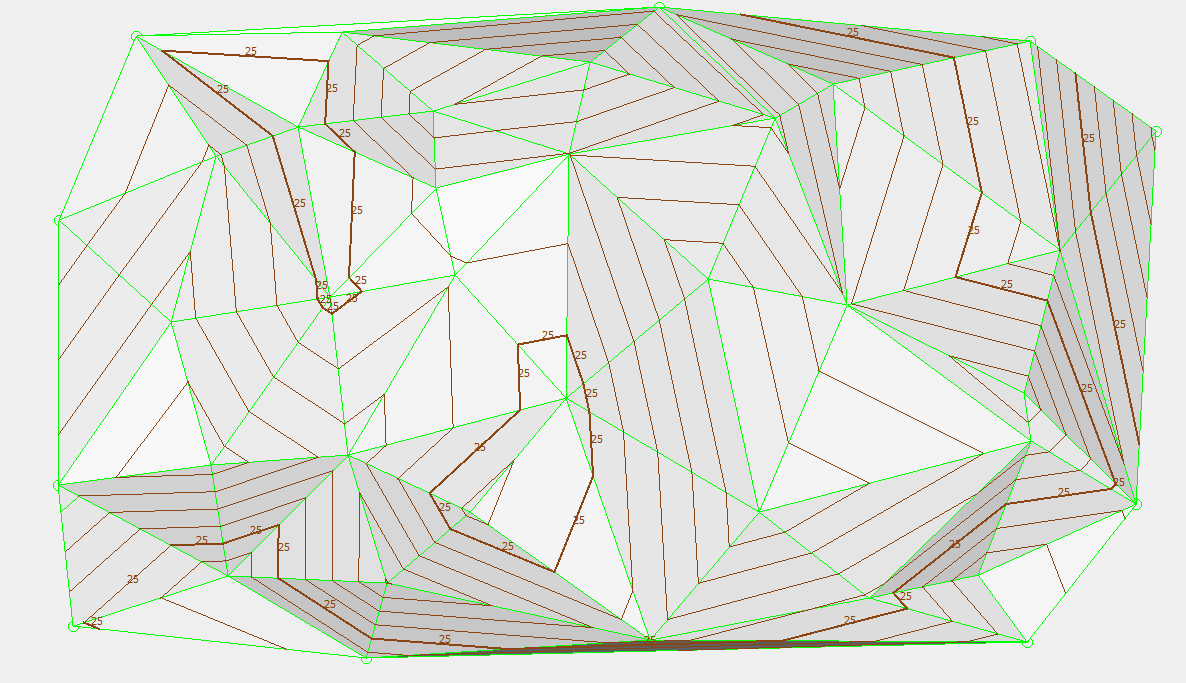
\includegraphics[width=15cm]{pictures/dtm_panchromatic_slope.PNG} 
\caption[Analýza sklonu v panchromatické škále nad body označenými kursorem myši]{Analýza sklonu v panchromatické škále nad body označenými kursorem myši}
\label{fig:dtm_panchromatic_slope}
\end{center}
\end{figure}

\vspace{0.2cm}
\begin{figure}[hbt!] 
\begin{center}
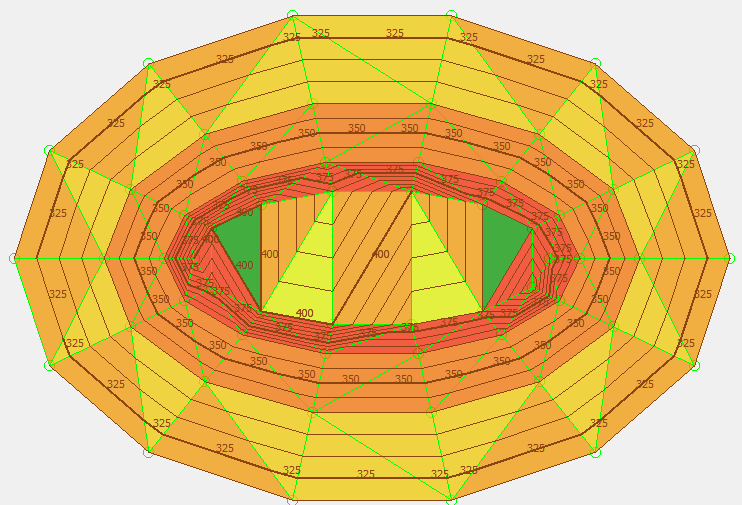
\includegraphics[width=13cm]{pictures/hill_colorful_slope.PNG} 
\caption[Analýza sklonu nad kupou v barevné škále]{Analýza sklonu nad kupou v barevné škále}
\label{fig:hill_colorful_slope}
\end{center}
\end{figure}

\vspace{0.2cm}
\begin{figure}[hbt!] 
\begin{center}
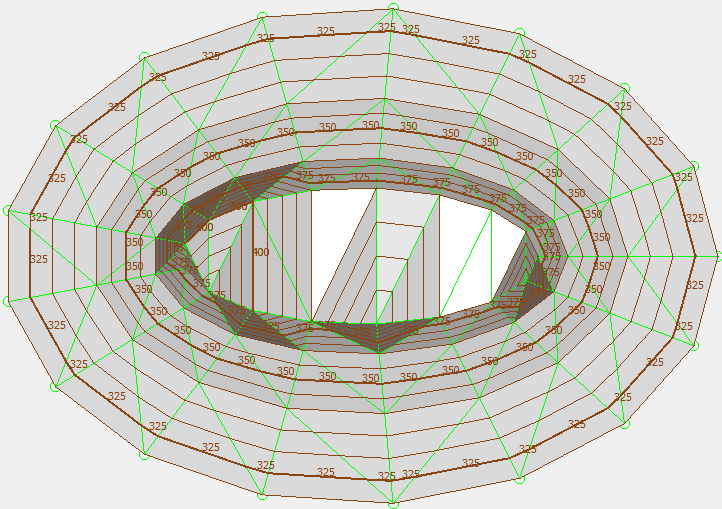
\includegraphics[width=14cm]{pictures/hill_panchromatic_slope.PNG} 
\caption[Analýza sklonu nad kupou v panchromatické škále]{Analýza sklonu nad kupou v panchromatické škále}
\label{fig:hill_panchromatic_slope}
\end{center}
\end{figure}

\vspace{0.2cm}
\begin{figure}[hbt!] 
\begin{center}
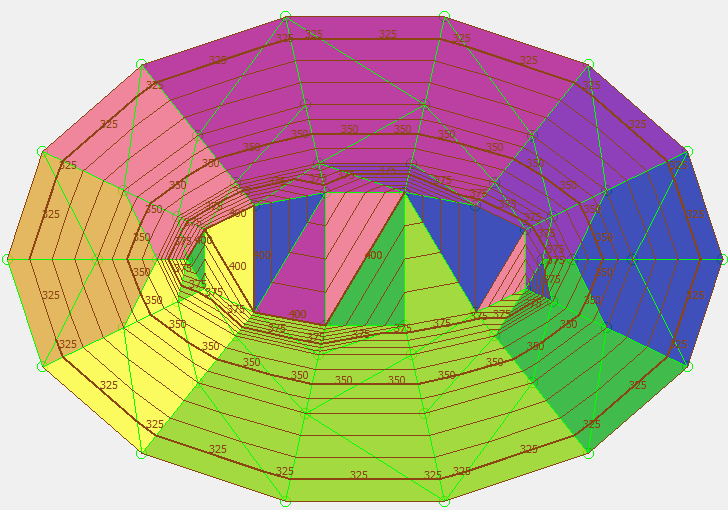
\includegraphics[width=13cm]{pictures/hill_colorful_aspect.PNG} 
\caption[Analýza expozice nad kupou v barevné škále]{Analýza expozice nad kupou v barevné škále}
\label{fig:hill_colorful_aspect}
\end{center}
\end{figure}

\vspace{0.2cm}
\begin{figure}[hbt!] 
\begin{center}
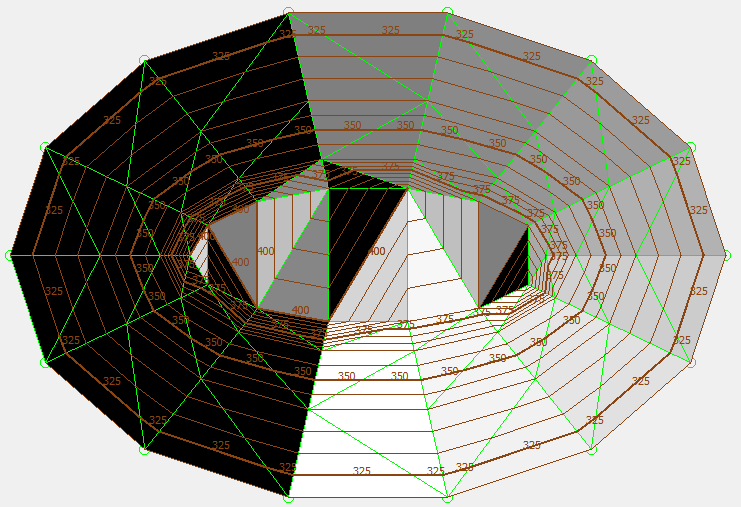
\includegraphics[width=14cm]{pictures/hill_panchromatic_aspect.PNG} 
\caption[Analýza expozice nad kupou v panchromatické škále]{Analýza expozice nad kupou v panchromatické škále}
\label{fig:hill_panchromatic_aspect}
\end{center}
\end{figure}


\vspace{0.2cm}
\begin{figure}[hbt!] 
\begin{center}
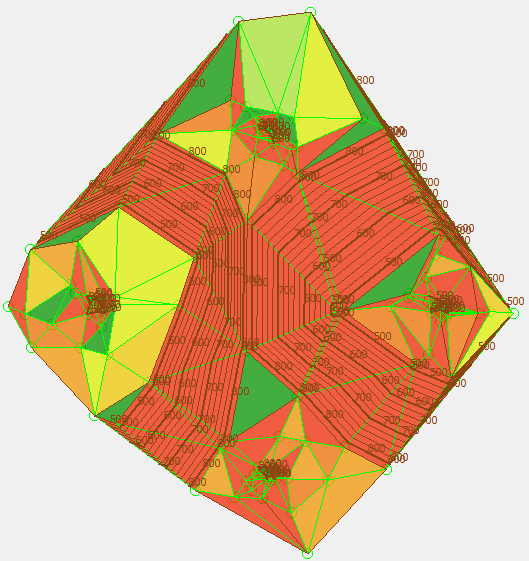
\includegraphics[width=9cm]{pictures/saddle_colorful_slope.PNG} 
\caption[Analýza sklonu nad sedlem v barevné škále]{Analýza sklonu nad sedlem v barevné škále}
\label{fig:saddle_colorful_slope}
\end{center}
\end{figure}

\vspace{0.2cm}
\begin{figure}[hbt!] 
\begin{center}
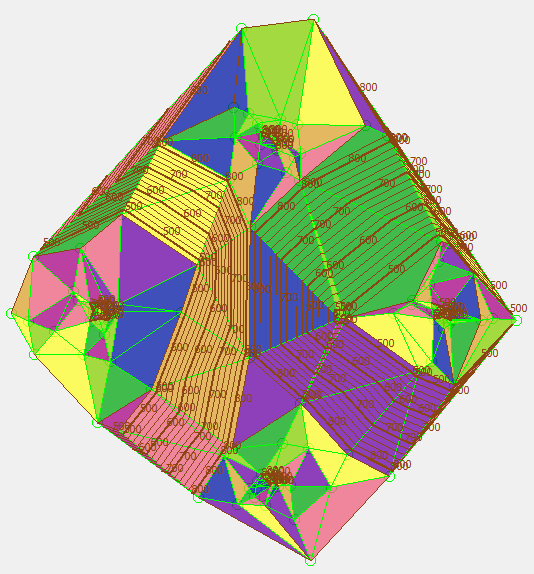
\includegraphics[width=9cm]{pictures/saddle_colorful_aspect.PNG} 
\caption[Analýza expozice nad sedlem v barevné škále]{Analýza expozice nad sedlem v barevné škále}
\label{fig:saddle_colorful_aspect}
\end{center}
\end{figure}

\vspace{0.2cm}
\begin{figure}[hbt!] 
\begin{center}
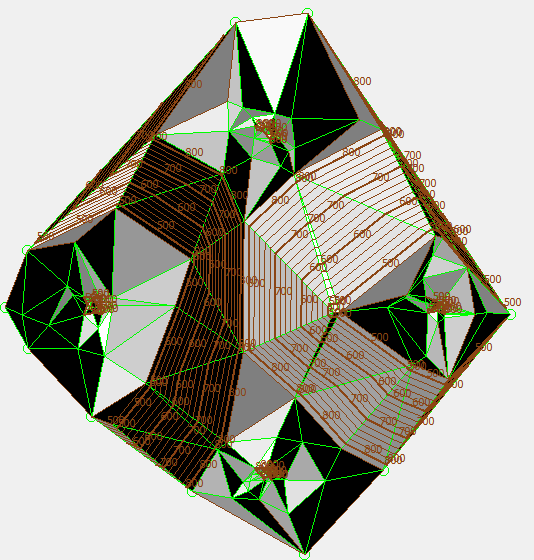
\includegraphics[width=10cm]{pictures/saddle_panchromatic_aspect.PNG} 
\caption[Analýza expozice nad sedlem v panchromatické škále]{Analýza expozice nad sedlem v panchromatické škále}
\label{fig:saddle_panchromatic_aspect}
\end{center}
\end{figure}

\vspace{0.2cm}
\begin{figure}[hbt!] 
\begin{center}
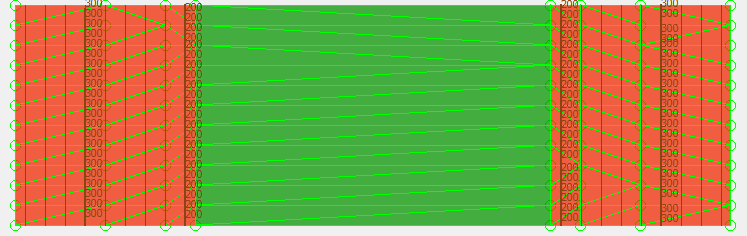
\includegraphics[width=11cm]{pictures/valley_colorful_slope.PNG} 
\caption[Analýza sklonu nad údolím v barevné škále]{Analýza sklonu nad údolím v barevné škále}
\label{fig:valley_colorful_slope}
\end{center}
\end{figure}

\vspace{0.2cm}
\begin{figure}[hbt!] 
\begin{center}
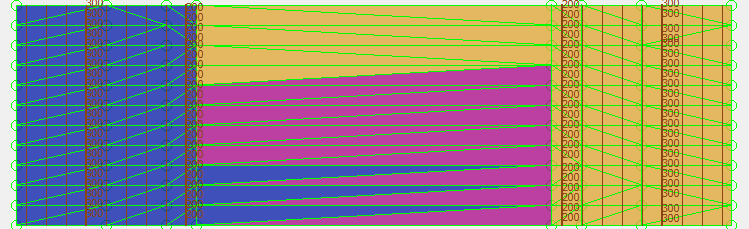
\includegraphics[width=11cm]{pictures/valley_colorful_aspect.PNG} 
\caption[Analýza expozice nad údolím v barevné škále]{Analýza expozice nad údolím v barevné škále}
\label{fig:valley_colorful_aspect}
\end{center}
\end{figure}

\vspace{0.2cm}
\begin{figure}[hbt!] 
\begin{center}
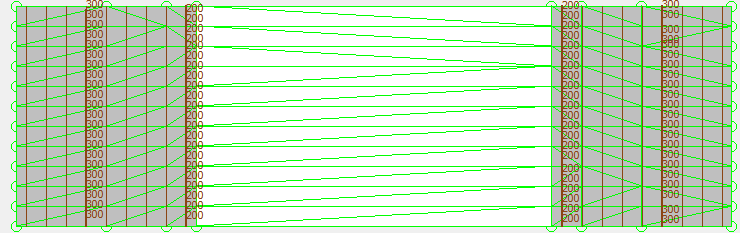
\includegraphics[width=13cm]{pictures/valley_panchromatic_slope.PNG} 
\caption[Analýza sklonu nad údolím v panchromatické škále]{Analýza sklonu nad údolím v panchromatické škále}
\label{fig:valley__panchromatic_slope}
\end{center}
\end{figure}

\vspace{0.2cm}
\begin{figure}[hbt!] 
\begin{center}
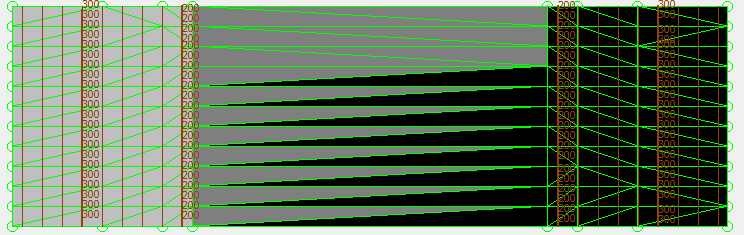
\includegraphics[width=13cm]{pictures/valley_panchromatic_aspect.PNG} 
\caption[Analýza expozice nad údolím v panchromatické škále]{Analýza expozice nad údolím v panchromatické škále}
\label{fig:valley_panchromatic_aspect}
\end{center}
\end{figure}

\vspace{0.2cm}
\begin{figure}[hbt!] 
\begin{center}
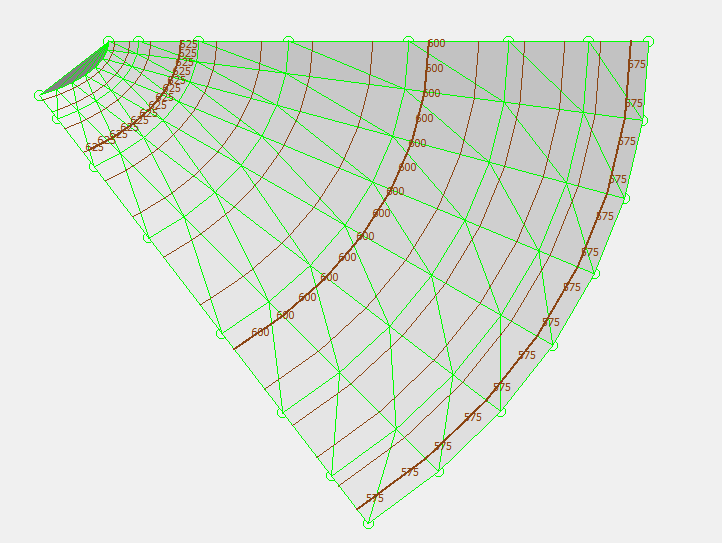
\includegraphics[width=12cm]{pictures/gentle_ridge_panchromatic_aspect.PNG} 
\caption[Analýza expozice nad spočinkem v panchromatické škále]{Analýza expozice nad spočinkem v panchromatické škále}
\label{fig:gentle_ridge_panchromatic_aspect}
\end{center}
\end{figure}

%% -------<<< 6. KAPITOLA = Technická dokumentace >>>-------\\%%

\newpage
\fancyhead[RE, RO]{\fancyplain{}{\small \sl{TECHNICKÁ DOKUMENTACE}}}

\vspace*{-1cm}
\section{Technická dokumentace}

\subsection{Třídy}
V aplikaci se nachází celkem sedm tříd - Algorithms, Draw, Generator, SortbyX, Edge, QPoint3D, Triangle a Widget. 

\subsubsection{Algorithms}
Třída Algorithms je nejobsáhlejší. Obsahuje konstruktor a dalšich několik pomocných i hlavních metod, které jsou určeny pro výpočet algoritmů používaných v digitálním GIS. \\

\noindent\textbf{int getPointLinePosition(QPoint3D \&q, QPoint3D \&p1, QPoin3D \&p2)}\\
Tato funkce má za úkol určit polohu bodu \textit{q} vůči přímce zadané dvěma body \textit{p1} a \textit{p2}. Z vektorů je vypočten determinant. Pokud je determinant větší než 0, bod se nechází v levé polorovině a funkce vrací hodnotu \textit{1}. Pokud je menší než 0, bod se nachází v pravé polorovině a funkce vrací hodnotu \textit{0}.  Pokud nenastane ani jeden z výše uvedených případů, tedy bod leží na linii, výstupem je hodnota \textit{-1}.\\

\noindent\textbf{double distance2Points(QPoint3D p1, QPoint3D p2)}\\
Metoda, jejíž návratová hodnota je typu double, vrací velikost spojnice mezi dvěma body.\\

\noindent\textbf{double getCircleRadius(QPoint3D \&p1, QPoint3D \&p2, QPoint3D \&p3, QPoint3D \&c)}\\
Metoda jejíž návratová hodnota je typu double, vrací velikost poloměru kružnice tvořené třemi vstupními body.\\

\noindent\textbf{int getNearestpoint(QPoint3D \&p, std::vector\textless QPoint3D\textgreater \&points)}\\
Tato metoda slouží k nalezení indexu nejbližšího bodu z množiny points k bodu p.\\

\newpage
\noindent\textbf{int getDelaunayPoint(QPoint3D \&s, QPoint3D \&e, std::vector\textless QPoint3D \textgreater \&points)}\\
Tato metoda slouží k nalezení indexu bodu, který splňuje Delaunayho vlastnosti.\\

\noindent\textbf{std::vector\textless Edge \textgreater DT(std::vector \textless QPoint3D \textgreater \&points)}\\
Metoda vytváří nad vektorem bodů Delaunayho triangulaci, která je reprezentována jako vektor hran.\\

\noindent\textbf{QPoint3D getContourPoint(QPoint3D \&p1, QPoint3D \&p2, double z)}\\
Metoda vypočte průsečík hrany, která je tvořena 3D body p1 a p2, s rovinou definovanou Z souřadnicí.\\

\noindent\textbf{std::vector\textless Edge \textgreater createContourLines(std::vector\textless Edge \textgreater \&dt, double z\_min, double z\_max, double dz, std::vector\textless int \textgreater \&contour\_heights)}\\
Metoda z triangulace dt v zadaném intervalu v ose Z $<z_{min} ; z_{max}>$ s intervalem vrstevnic dz vrátí vektor hran definující vrstevnice. Aby bylo možné vytvořit popis vrstevnic, je v rámci této funkce sestavován i vektor výšek typu integer. \\

\noindent\textbf{double calculateSlope(QPoint3D \&p1, QPoint3D \&p2, QPoint3D \&p3)}\\
Tato metoda slouží k vypočetní hodnoty sklonu v trojúhelníku definovaném 3D body p1, p2 a p3.\\

\noindent\textbf{double calculateAspect(QPoint3D \&p1, QPoint3D \&p2, QPoint3D \&p3)}\\
Tato metoda slouží k vypočetní hodnoty expozice v trojúhelníku definovaném 3D body p1, p2 a p3.\\

\noindent\textbf{std::vector\textless Triangle\textgreater analyzeDTM(std::vector\textless Edge \textgreater \&dt)}\\
Metoda prochází jednotlivé trojúhelníky Delaunayho triangulace a počítá analýzu sklonu a expozice. \\

\newpage
\vspace*{-1cm}
\subsubsection{Generator}
Tato třída obsahuje algoritmy pro automatické generování terénních tvarů.Vstupem do těchto algoritmů je šířka a výška zobrazovacího widgetu.\\

\noindent\textbf{std::vector\textless QPoint3D\textgreater generateHill(int width, int height)}\\
Tvorba kupy.\\

\noindent\textbf{std::vector\textless QPoint3D\textgreater generateValley(int width, int height))}\\
Tvorba údolí.\\

\noindent\textbf{std::vector\textless QPoint3D\textgreater generateRidge(int width, int height)}\\
Tvorba hřbetu.\\

\noindent\textbf{std::vector\textless QPoint3D\textgreater generateSaddle(int width, int height))}\\
Tvorba sedla.\\

\noindent\textbf{std::vector\textless QPoint3D\textgreater generateGentleRidge(int width, int height))}\\
Tvorba spočinku.\\

\noindent\textbf{std::vector\textless QPoint3D\textgreater generateGrid(int size))}\\
Tvorba čtvercového gridu, vstupem je vzdálenost bodů.\\

\subsubsection{Draw}

Třída Draw obsahuje několik metod. Metody jsou určeny pro generování a vykreslování proměnných.\\

\noindent\textbf{void paintEvent(QPaintEvent *e)}\\
Nejobsáhlejší metoda sloužcíí k vykreslení bodů a zobrazení výsledků použitých algoritmů.\\

\noindent\textbf{void mousePressEvent(QMouseEvent *e)}\\
Metoda uloží bod se souřadnicemi místa kliknutí v zobrazovacím okně a dá tomuto bodu náhodou souřadnici z.\\

\noindent\textbf{void setPoints(std::vector\textless QPoint3D \textgreater points\_)}\\
Metoda slouží pro nastavení privátní položky \textit{points}, tak aby byla vidět v třídě Draw.\\

\noindent\textbf{std::vector\textless QPoint3D \textgreater \& getPoints()}\\
Metoda slouží pro vrácení privátní položky \textit{points} z třídy Draw.\\

\noindent\textbf{std::vector\textless Edge \textgreater \& setDT()}\\
Metoda slouží pro nastavení privátní položky \textit{dt}, tak aby byla vidět z třídy Draw.\\

\noindent\textbf{void getDT(std::vector\textless Edge\textgreater \&dt\_)}\\
Metoda slouží pro vrácení privátní položky \textit{dt} z třídy Draw. \\

\noindent\textbf{std::vector\textless Edge \textgreater \& getDTsize()}\\
Metoda slouží pro vrácen velikosti Delaunayho triangulace z třídy Draw.\\

\noindent\textbf{void setContours(std::vector\textless Edge\textgreater\&contours\_, std::vector\textless int\textgreater\&contour\_heights, int dz\_)}\\
Metoda slouží pro nastavení privátních položek týkajících se vrstevnic, tak aby byly vidět v třídě Draw.\\

\noindent\textbf{std::vector\textless Edge\textgreater \& getContours()}\\
Metoda slouží pro převod vrstevnic do vykreslovacího okna.\\

\noindent\textbf{void setMainContours(std::vector\textless Edge\textgreater\&mainContours\_, std::vector\textless int\textgreater\&main\_contour\_heights, int main\_dz\_)}\\
Metoda slouží pro nastavení privátních položek týkajících se hlavních vrstevnic, tak aby byly vidět v třídě Draw.\\

\noindent\textbf{std::vector\textless Edge\textgreater \& getMainContours()}\\
Metoda slouží pro převod hlavních vrtevnic do vykreslovacího okna.\\

\noindent\textbf{void setSlope(bool slope\_)}\\
Metoda slouží jako podmínka TRUE/FALSE pro vykreslení sklonu terénu.\\

\noindent\textbf{void setAspect(bool aspect\_)}\\
Metoda slouží jako podmínka TRUE/FALSE pro vykreslení expozice terénu.\\

\noindent\textbf{void setDTM(std::vector\textless Triangle\textgreater \&dtm\_)}\\
Metoda slouží pro  nastavení privátních položek týkajících se trojúhelníků a jejich informací o sklonu a expozici terénu.\\

\noindent\textbf{void importPolygons(std::string \&path, std::vector\textless QPoint3D \textgreater \&points,  QSizeF \&canvas\_size, double \&min\_z, double \&max\_z)}\\
Tato metoda slouží pro import bodů ze souboru. Z cesty path se naplní vektor points a uloží hodnotu s minimální a maximální souřadnicí. Proměnná canvas\_size slouží k vykreslení v rozsahu importovaných dat.\\

\noindent\textbf{void clearDT()}\\
Metoda slouží k vymazání celého obsahu okna a k překreslení.\\

\noindent\textbf{void clearPoints()}\\
Metoda slouží pouze k vymazání bodů.\\

\subsubsection{SortbyX}

Tato jednoduchá třída slouží k setřídění vstupního pole souřadnic podle osy x.\\

\noindent\textbf{bool operator()(QPoint \&p1, QPoint \&p2)}\\
Přetížený operátor () vrátí bod s větší souřadnicí x z dvojice bodů.\\

\newpage
\vspace*{-1cm}
\subsubsection{Edge}

\noindent\textbf{Edge(QPoint3D \&start, QPoint3D \&end)}\\
Třída Edge je zkonstruována ze dvou 3D bodů, počátku a konce hrany. Třída slouží k uložení hrany triangulace i vrstevnice.\\
    
\noindent\textbf{QPoint3D \&getStart()}\\
Metoda vrátí počáteční bod hrany.\\

\noindent\textbf{void setStart(QPoint3D \& s)}\\
Metoda nastaví počáteční bod hrany.\\

\noindent\textbf{QPoint3D \& getEnd()}\\
Metoda vrátí koncový bod hrany.\\

\noindent\textbf{void setEnd(QPoint3D \& e)}\\
Metoda nastaví koncový bod hrany.\\

\noindent\textbf{void changeOrientation()}\\
Metoda prohodí orientaci hrany.

\subsubsection{QPoint3D}

\noindent\textbf{QPoint3D(double x, double y, double z\_)}\\
Třída QPoint3D je odvozena z třídy QPointF a složí k uložení bodu s informací o výšce.\\

\noindent\textbf{double getZ()}\\
Metoda vrátí výšku bodu.\\

\noindent\textbf{void setZ(double z\_)}\\
Metoda nastaví výšku bodu.

\newpage
\vspace*{-1cm}
\subsubsection{Triangle}

\noindent\textbf{Triangle(QPoint3D \&p1\_, QPoint3D \&p2\_, QPoint3D \&p3\_, double slope\_, double aspect\_))}\\
Třída QPoint3D složí k uložení trojúhelníku definovaného body p1, p2, p3 a jeho informace o sklonu a expozici.\\

\noindent\textbf{ QPoint3D getP1()}\\
Metoda vrátí první bod trojúhelníku.\\

\noindent\textbf{ QPoint3D getP2()}\\
Metoda vrátí druhý bod trojúhelníku.\\

\noindent\textbf{ QPoint3D getP3()}\\
Metoda vrátí třetí bod trojúhelníku.\\

\noindent\textbf{double getSlope()}\\
Metoda vrátí sklon trojúhelníku.\\

\noindent\textbf{double getAspect()}\\
Metoda vrátí expozici trojúhelníku.\\

\noindent Obdobně jako gettery byly nastaveny settery.

\subsubsection{Widget}

\noindent\textbf{void on\_createDelaunay\_clicked()}\\
Při stisknutí tohoto tlačítka se zavolá metoda třídy Algorithms DT a výsledek se zobrazí v okně. \\

\noindent\textbf{void on\_clearDT\_clicked()}\\
Při stisknutí tlačítka Clear DT se zavolá metoda třídy Draw clearDT a smaže se celý obsah okna.\\

\noindent\textbf{void on\_clearPoints\_clicked()}\\
Při stisknutí tlačítka Clear points se smažou body.\\

\noindent\textbf{void on\_createContours\_clicked()}\\
Při stisknutí tlačítka Create Contours se zkontroluje, zda byla již vytvořena DT. Pokud ne, vytvoří se a nad ní se poté zavolá metoda třídy Algorithms createContours a výsledek se zobrazí v okně.\\

\noindent\textbf{void on\_importPolygons\_clicked()}\\
Při stisknutí tlačítka Import, se otevře okno pro výběr importovaných dat. \\

\noindent\textbf{void on\_analyzeDTM\_clicked()}\\
Při stisknutí tlačítka AnalyzeDTM se zavolá metoda třídy Algorithms analyzeDTM a podle vybrané analýzy v ComboBoxu se zobrazí v okně buď analýza sklonu, nebo expozice. \\

\noindent\textbf{void on\_generateTerrain\_clicked()}\\
Při stisknutí tlačítka Generate a výběru z comboboxu se vygenerují body terénu.\\

\noindent\textbf{void on\_Save\_clicked()}\\
Při stisknutí tlačítka Save, se otevře okno pro volbu místa uložení vytvořeného obrázku a následně je obrázek uložen.



%% -------<<< 7. KAPITOLA = Závěr >>>-------\\%%
\newpage
\fancyhead[RE, RO]{\fancyplain{}{\small \sl{DISKUSE}}}

\vspace*{-1cm}
\section*{Diskuse}
\addcontentsline{toc}{section}{Diskuse}
V této části se zamyslíme nad slabostmi použitých algoritmů a nad možnými vylepšeními. \\

\noindent\textbf{Delaunayho triangulace}\\
\noindent Algoritmus DT není jednoznačný pro body na mřížce. Zároveň selhává pro některé terénní tvary (zejména sedlo). Oba tyto problémy by se daly vyřešit triangulací se vstupní podmínkou, která definuje povinné hrany, jež umožňují lepší modelování morfologie terénu. V aplikaci není bohužel možné definovat povinné hrany, proto program není dost dobře použitelný pro data se složitějšími typy terénních tvarů. Tvorba povinných hran by výrazně zkvalitnila aplikaci, neboť by uživatel získával věrohodnější výstupy. S tímto problémem souvisí i to, že jsou následně chybně vykresleny vrstevnice. V rámci úlohy nebyla řešena triangulace nekonvexní oblasti. Tedy i na místech, kde už nejsou podrobné body jsou chybně vytvářeny trojúhelníky. Aplikace je tedy užitečná pro málo členitá výškopisná data v terénu bez povinných hran, například spočinek je zobrazen velmi věrohodně.\\

\noindent\textbf{Import dat}\\
\noindent Při importu není řešen souřadnicový systém dat. Body by před nahráním do mapového okna měly být transformovány do takového souřadnicového systému, který data vhodně zobrazí. V této úloze se však primárně zabýváme tvorbou digitálního modelu, není tedy na transformaci vstupních dat brán ohled. V testovaném souboru jsou jen takové body, které se v rozhraní správně vykreslí. \\

\noindent\textbf{Vykreslení vrstevnic}\\
\noindent Pro vykreslení vrstevnic byl použit lineární interpolační algoritmus, který předpokládá, že spád mezi dvěma body, mezi nimiž provádíme interpolaci, je konstantní. Tento algoritmus je sice výpočetně jednoduchý, ale nevystihuje realitu. Pro kvalitní výsledek by bylo vhodnější použít geomorfologickou interpolaci, která předpokládá plynulou změnu sklonu terénu mezi jednotlivými body. Tento typ interpolace se však obtížně algoritmizuje, často je tvořena ručně zkušenými kartografy.\\
\indent Pokud se zaměříme na vrstevnice, pro údolí a hřbet jsou vykresleny korektně. U vrstevnic kupy již dochází k chybám a to zejména blízko vrcholu. Důvodem je, že body jsou na kružnici, kde Delaunayho triangluace není jednoznačná. Vrstevnice mají zvláštní tvar, někdy se dokonce i kříží, případně dvojí. Velmi zle jsou vrstevnice generovány u sedla, kde blízko vrcholů a prohlubní vytváří maličké uzavřené polygonky a dál od nich chybí úplně. Vrstevnice by se měly chovat rovnoměrně, lahodit oku, což v případě sedlového útvaru rozhodně neplatí.\\
\indent Špatně vykreslené vrstevnice jsou zřejmé z následujících obrázků:\\

\vspace{0.2cm}
\begin{figure}[hbt!] 
\begin{center}
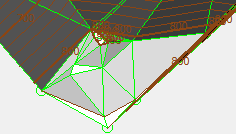
\includegraphics[width=10cm]{pictures/saddle_panchromatic_slope_detail.PNG} 
\caption[Chybné vrstevnice při analýze sklonu nad sedlem]{Chybné vrstevnice při analýze sklonu nad sedlem}
\label{fig:saddle_panchromatic_slope_detail}
\end{center}
\end{figure}

\vspace{0.2cm}
\begin{figure}[hbt!] 
\begin{center}
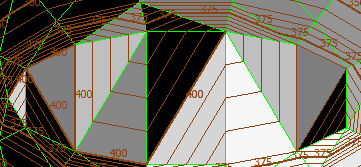
\includegraphics[width=10cm]{pictures/hill_panchromatic_aspect_detail2.PNG} 
\caption[Chybné vrstevnice při analýze expozice nad kupou]{Chybné vrstevnice při analýze expozice nad kupou}
\label{fig:hill_panchromatic_aspect_detail2}
\end{center}
\end{figure}

\newpage
\noindent\textbf{Výpočet a vykreslení sklonu a expozice}\\
Může vzniknout problém v rovinatém území, jak je patrné z obrázku \ref{fig:hill_colorful_slope}. Při výpočtu vznikají zaokrouhlovací chyby, které se promítnou do sklonu a expozice. Proto se terén jeví uživateli jako nerovinný.\\
\indent Při vykreslení sklonu terénu byly pro ilustraci zvoleny odstíny od zelené po červenou. Sklon nabývá hodnot od 0 do 180 $^\circ$, nicméně reálně jsou hodnoty sklonu o dost nižší, proto byla barevná stupnice volena v intervalu od 1 $^\circ$ do 22 $^\circ$. \\
\indent Vykreslení expozice bylo rovněž obohaceno o barevnou semi-průhlednou paletu, jež byla také odvozena od palety z aplikace Analýzy výškopisu. Výsledná směrnice byla rozdělena do osmi směrů - S, SV, V, JV, J, JZ, Z, SZ. Rovina uvažována nebyla. Byla snaha o velkou barevnou návaznost, aby byl výsledný obrázek přehledný. Nicméně i přesto by bylo rozhodně vhodné u obou analýz do mapového okna doplnit legendu. \\ 
\indent V aplikaci je možné si vybrat i panchromatickou paletu, nicméně zvláště pro vykreslení expozice není tato paleta vhodná, viz \ref{fig:hill_panchromatic_aspect_detail}. Mezi černou a bílou barvou je nepěkný kontrast, lepší je využít barevnou stupnici, která na sebe ve všech barvách navazuje.\\
\indent Chybné nebo nedostatečně přesné analýzy jsou zřejmé z následujících obrázků:\\

\vspace{0.2cm}
\begin{figure}[hbt!] 
\begin{center}
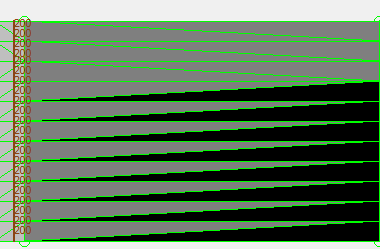
\includegraphics[width=11cm]{pictures/valley_panchromatic_aspect_detail.PNG} 
\caption[Nejednoznačnost DT ve středové části údolí]{Nejednoznačnost DT ve středové části údolí}
\label{fig:valley_panchromatic_aspect_detail}
\end{center}
\end{figure}

\vspace{0.2cm}
\begin{figure}[hbt!] 
\begin{center}
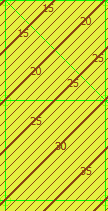
\includegraphics[width=5cm]{pictures/grid_colorful_slope_detail.PNG} 
\caption[Nejednoznačnost DT u gridu]{Nejednoznačnost DT u gridu}
\label{fig:grid_colorful_slope_detail}
\end{center}
\end{figure}

\vspace{0.2cm}
\begin{figure}[hbt!] 
\begin{center}
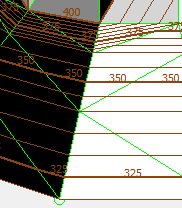
\includegraphics[width=7cm]{pictures/hill_panchromatic_aspect_detail.PNG} 
\caption[Nevhodná škála při analýze expozice nad kupou]{Nevhodná škála při analýze expozice nad kupou}
\label{fig:hill_panchromatic_aspect_detail}
\end{center}
\end{figure}

\indent Vyhodnocení sklonu i expozice terénu je stejně jako vykreslení vrstevnic v některých případech velmi nejednoznačné. Pro hřbet i údolí je sklon zobrazen správně. Znázornění spočinku je také správné, je krásně patrné, jak směrem dolů rozestup vrstevnic roste a pak se zase snižuje. Pro kupu je nekorektně vyobrazen střed, neboť v něm nejsou korektně vykresleny Delaunay trojúhelníky. Obdobný problém pak platí u sedla. Expozice pro údolí a hřbet je ve středové části chybná (viz obrázek \ref{fig:valley_colorful_aspect}), nastává stejný problém, jako při generování gridu, kdy DT je nejednoznačná. \\
Co se týče importovaných dat, textové soubory neobsahují mnoho výrazných terénní útvarů, které by mohly ovlivnit výpočty. Vrstevnice, sklon i expozice byly pro importovaná data vykresleny víceméně správně (když vezmeme v úvahu lineární interpolaci, přesnější by byla samozřejmě morfologická). 

\newpage
\vspace*{-1cm}
\fancyhead[RE, RO]{\fancyplain{}{\small \sl{ZÁVĚR}}}
\section*{Závěr}
\addcontentsline{toc}{section}{Závěr}
\noindent
\large
Byla vytvořena aplikace, která má několik funkcionalit. Umí generovat vybrané terénní tvary, importovat soubor se souřadnicemi i kreslit body kursorem myši. Nad všemi těmito množinami dokáže zkonstruovat Delaunay triangulaci, jejíž trojúhelníky jsou ztěžejní při následném generování vrstevnic a provádění analýz sklonu a expozice. Dále má uživatel možnost uložit si vytvořený model jako obrázek, což může výrazně pomoci při práci. V rámci bonusových úloh byly vytvořeny některé terénní útvary, konkrétně kupa, hřbět, sedlo, údolí a spočinek. Co se týče výstupů aplikace, pro některé útvary funguje kód korektně, pro jiné se vyskytují chyby. Ukázky jednotlivých výsledků lze nalézt v kapitole 6. Pro kvalitnější výsledek by bylo vhodné použít nějakou funkci pro vyhlazení vrstevnic či pro tvorbu vrstevnic prostřednictvím morfologické interpolace.\\
\indent I přesto, že se mnoho věcí podařilo do aplikace naprogramovat, je nespočet funkcionalit, které jsou velmi podstatné a v aplikaci chybí. Jednou z hlavních je zobrazení jednotlivých vrstevnic podle kartografických zásad. Z vygenerované nebo importované množiny bodů není možné odstranit některé body, nad kterými nechci provádět analýzu, nebo vybrat zájmovou oblast pomocí ohraničujícího obdélníku. Dalším vylepšením by byla například schopnost generovat správně DT v nekonvexní oblasti, či umožnit kromě zobrazení vrstevnic i barevnou hypsometrii nebo 3D vizualizaci terénu.




%% -------<<< LITERATURA >>>-------\\%%
\newpage
\vspace*{-6ex}
\renewcommand{\refname}{Literatura} 
\fancyhead[RE, RO]{\fancyplain{}{\small \sl{LITERATURA}}}
    \bibliographystyle{czechiso}
    \bibliography{literatura}
 
\end{document}


